\documentclass[11pt,a4paper]{article}
\usepackage[T1]{fontenc}
\usepackage[utf8]{inputenc}
\usepackage{lmodern}
\usepackage[margin=2cm]{geometry}
\usepackage{graphicx,booktabs,tabularx,longtable,array,xcolor,enumitem}
\usepackage[hidelinks]{hyperref}
\setlist{nosep,leftmargin=1.2em}
\renewcommand{\arraystretch}{1.12}
\newcolumntype{Y}{>{\raggedright\arraybackslash}X}
\newcolumntype{P}[1]{>{\raggedright\arraybackslash}p{#1}}
\setlength{\parindent}{0pt}\setlength{\parskip}{4pt}
\sloppy

\begin{document}
\begin{center}
{\Large\bfseries 23CSE455 Design Patterns}\\[2pt]
{\large Case Study Report}
\end{center}

\textbf{Team:} A6\\
\textbf{Case study:} Ride-Sharing Application using Node.js/Express -- \emph{Design Pattern Analysis in a Node.js/Express Ride-Sharing Application}\\
\textbf{Application:} Sarathi backend (TypeScript, Express 4) -- \url{https://github.com/AkhilMM2000/sarathi-backend}; faculty approval confirmed (reported by the team lead).\\
\textbf{Date:} 2026-10-11\\
\textbf{Submission repository:} 23CSE455\_DP\_CaseStudy

\textbf{Students}\\
\begin{tabular}{@{}lll@{}}\toprule Roll number & Student name & Batch\\\midrule
AM.SC.U4CSE23137 & Dilip Kumar Reddy & CSE B \\
AM.SC.U4CSE23326 & Sai Sameer & CSE D \\
AM.SC.U4CSE23134 & M Kumar & CSE B \\
AM.SC.U4CSE23129 & K Harish & CSE B \\
AM.SC.U4CSE23154 & S Leela Shankar & TO FILL \\
\bottomrule\end{tabular}

%=====================================================================
\section{Application and architecture}
\textbf{Original source:} \url{https://github.com/AkhilMM2000/sarathi-backend}, default branch, baseline commit
\texttt{c8766f4c88b9f36235d5f4399ef9b4cf20df3c8a} (2026-06-16, 185 commits), accessed 2026-10-11.
\textbf{License:} the repository has no LICENSE file (\texttt{package.json} declares ISC); it is used here only for academic analysis.

\textbf{Environment:} TypeScript 5.9.3 on Node.js 22.18.0; Express 4.22; Mongoose 8.24 (MongoDB Atlas); tsyringe 4.10;
Socket.IO 4.8; Upstash Redis; Stripe 18.5; Google Distance Matrix API; Zod 4.6. Versions are those resolved by
\texttt{npm install} on 2026-10-11 because upstream ignores \texttt{package-lock.json}; with them \texttt{tsc --noEmit} reports 7
type errors, all in files we did not change (Stripe API-version literal, Express 5 typings, Upstash typings).

\textbf{Scope:} the seven areas of the case study -- rider, driver (incl.\ reviews), trip, payment (Stripe, Stripe Connect, wallet),
driver matching, location and notification -- plus the framework code they use (DI container, middleware, error handling).
Excluded as outside these areas: chat, vehicles, file upload, referral rewards, OTP/registration/OAuth/password reset, admin dashboards.
Excluded from the copied code: \texttt{dist/} (compiled output), screenshots, a compiler log; demo credentials in the README were redacted.

\textbf{Architecture:} the code follows a four-layer clean architecture (Figure~\ref{fig:arch}). A ride request enters
\texttt{index.ts}, passes the route's middleware chain (\texttt{protectRoute} $\rightarrow$ \texttt{CheckBlockedUserOrDriver}),
reaches \texttt{BookingController.bookDriver}, which validates the DTO with Zod and calls the \texttt{BookDriver} use case.
\texttt{BookDriver} computes the fare, asks \texttt{IDriverRepository} for approved drivers within 30\,km (MongoDB \texttt{\$geoNear}),
filters them to 20\,km road distance through \texttt{GoogleDistanceService}, saves a PENDING booking through \texttt{IBookingRepository}
and broadcasts \texttt{booking:new} through \texttt{INotificationService}, implemented by \texttt{SocketNotificationService}
(Redis maps driver id to socket id). The first driver to call \texttt{AcceptBooking} wins an atomic PENDING$\rightarrow$CONFIRMED update;
\texttt{CronScheduler} expires requests nobody accepts. All collaborators are wired by the tsyringe container.

\begin{figure}[h]\centering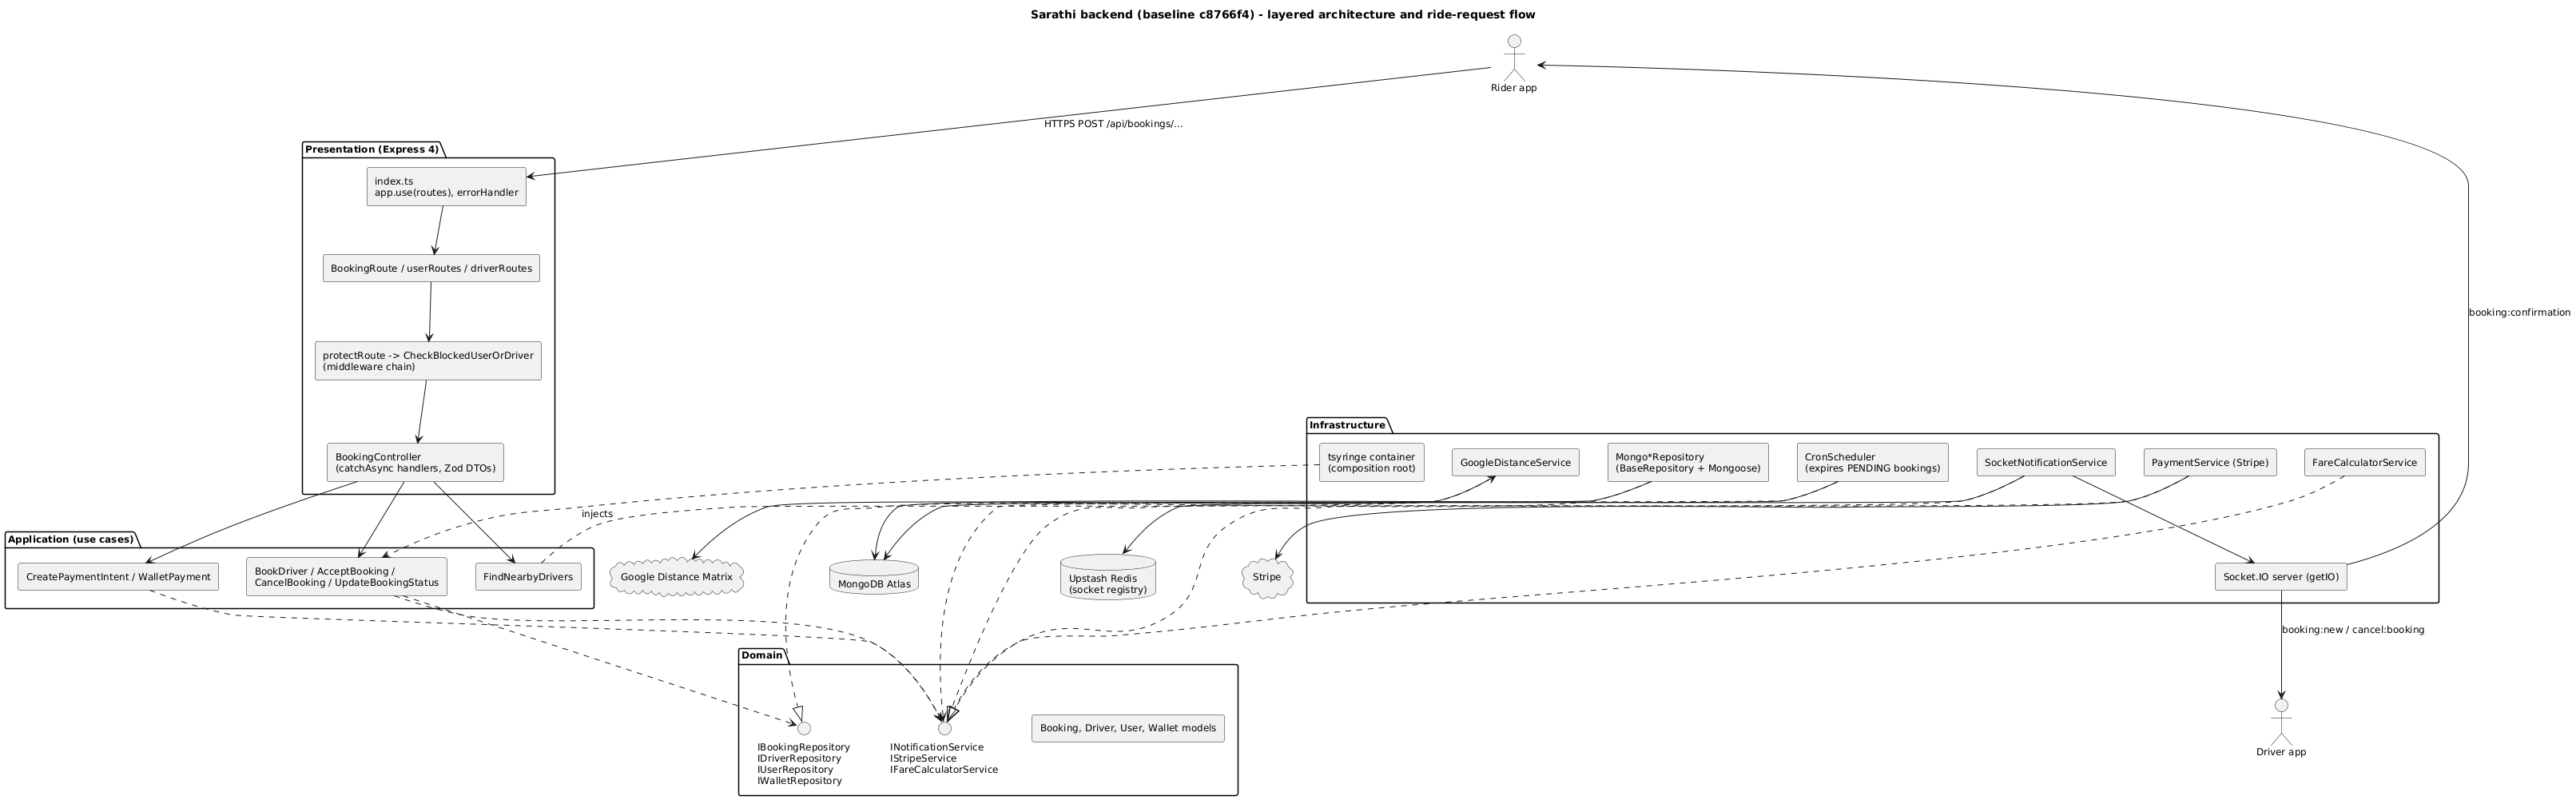
\includegraphics[width=\linewidth]{Part1/diagrams/architecture.png}
\caption{Layered architecture and ride-request flow (\texttt{Part1/diagrams/architecture.puml}).}\label{fig:arch}\end{figure}

\textbf{Run instructions:} \texttt{README.md}. Running the server needs MongoDB, Redis, Stripe and Google credentials, which we did not have,
so behaviour was verified through the real use-case classes with in-memory fakes: \texttt{cd Part2/code \&\& npm install \&\& npm test}.
Baseline characterization run (unchanged \texttt{src}, test files added): 14/14 passed (\texttt{Part1/evidence/test\_results.txt}).

%=====================================================================
\section{Part 1 Pattern discovery}
\textbf{Method:} (1) mapped the seven areas to files; (2) collected candidates from interfaces, DI registrations, naming and a first
LLM pass (Section~\ref{sec:llm}); (3) for every candidate traced implementers, injection points and call sites, and accepted it only
when the roles of the pattern are present and interact; (4) recorded rejected and uncertain candidates with a reason;
(5) wrote characterization tests for behaviour the changes would touch. A class name, decorator or LLM statement alone was never accepted.

\subsection{Totals at the baseline}
\textbf{Confirmed pattern types:} 10 -- Layered Architecture, Dependency Injection, Singleton, Repository, Data Mapper, Adapter,
Gateway, Observer, Chain of Responsibility, Decorator.\\
\textbf{Confirmed pattern instances:} 16.\\
\textbf{Concrete participant classes:} 11 (five Mongo repositories, \texttt{SocketNotificationService}, \texttt{PaymentService},
\texttt{StripeService}, \texttt{GoogleDistanceService}, \texttt{CheckBlockedUserOrDriver}, \texttt{BookingController}).\\
\textbf{Unique participant symbols:} 69 distinct classes, interfaces, functions and modules across all 16 records (shared symbols counted once; list in \texttt{Part1/evidence/participant\_symbols.txt}).\\
\textbf{Rejected and uncertain candidates:} 6 rejected, 2 uncertain (Table~\ref{tab:rej}); observation scope as above.

\subsection{Pattern inventory}
\begin{longtable}{@{}P{0.17\linewidth}P{0.5\linewidth}rr@{}}
\toprule Pattern type & Instance names & Instances & Concrete cl.\\\midrule\endhead
Layered Architecture & Ride Booking Request Flow & 1 & 0 \\
Dependency Injection & Use-Case and Service Composition Root & 1 & 0 \\
Singleton & Shared Socket.IO Server Instance & 1 & 0 \\
Repository & Trip Booking Repository; Driver Repository with Geospatial Matching Query; Rider Repository; Rider Wallet Ledger Repository; Driver Review Repository & 5 & 5 \\
Data Mapper & Driver Review Persistence Mapping & 1 & 0 \\
Adapter & Socket.IO Ride Notification Adapter; Stripe Ride Payment Adapter; Stripe Connect Driver Payout Onboarding Adapter & 3 & 3 \\
Gateway & Google Distance Matrix Location Gateway & 1 & 1 \\
Observer & Ride Event Notification & 1 & 0 \\
Chain of Responsibility & Authenticated Ride Request Pipeline & 1 & 1 \\
Decorator & Async Controller Error Forwarding & 1 & 1 \\
\bottomrule
\end{longtable}

\begin{longtable}{@{}P{0.2\linewidth}P{0.1\linewidth}P{0.62\linewidth}@{}}
\caption{Rejected and uncertain candidates (baseline).}\label{tab:rej}\\
\toprule Candidate & Verdict & Reason\\\midrule\endfirsthead
\toprule Candidate & Verdict & Reason\\\midrule\endhead
Strategy & rejected & FareCalculatorService: only one implementation of IFareCalculatorService; ride-type behaviour is an if/else inside calculate (infrastructure/services/FareCalculatorService.ts:20-36). An interface used for DI is not a family of interchangeable algorithms. \\
State & rejected & BookingStatus and driver status are enums/strings; transitions are scattered if-checks (CancelBooking.ts:35-51, UpdateBookingstatus.ts:36-63, AdminChangeDriverStatus.ts:24-33). No state objects. \\
Command & rejected & Use cases expose execute(), but there is no invoker storing, queuing or undoing command objects; controllers call them directly. Classified as use-case interactors inside the Layered Architecture. \\
Template Method & rejected & BaseRepository is a generic layer supertype with complete methods; it defines no algorithm skeleton with abstract/hook steps (BaseRepository.ts:5-41). \\
Factory Method & rejected & protectRoute(allowedRoles) returns a configured closure (authMiddleware.ts:15-18); there is no creator hierarchy deciding which product class to instantiate. \\
Facade & rejected & Controllers delegate to one use case per action; they do not simplify a subsystem of several collaborating classes. \\
Adapter (Google Maps road distance) & uncertain & GoogleMapService implements IGoogleMapService (GoogleMapService.ts:8-70) and is registered (container.ts:99-101) but no class in the code injects IGoogleMapService, so no Client participant exists. \\
Adapter (Twilio SMS) & uncertain & TwilioSMSService implements SMSService (TwilioSMSService.ts:6-16) and is registered (container.ts:65) but nothing resolves 'SMSService'; dormant code. \\
\bottomrule
\end{longtable}

\begin{figure}[h]\centering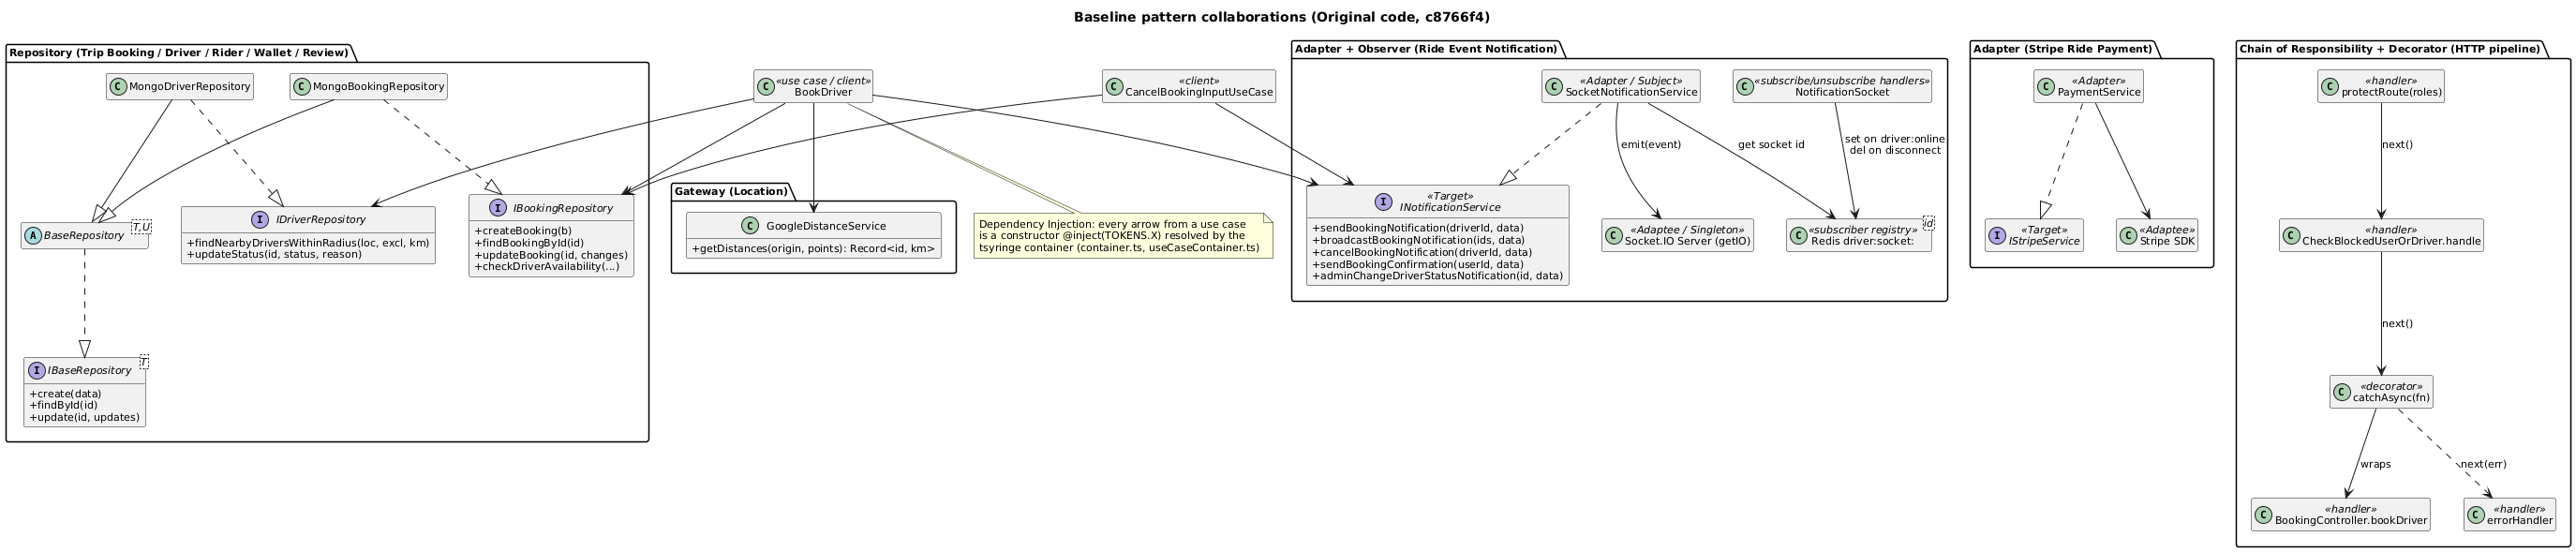
\includegraphics[width=\linewidth]{Part1/diagrams/baseline_patterns.png}
\caption{Main baseline collaborations (\texttt{Part1/diagrams/baseline\_patterns.puml}).}\end{figure}

\subsection{One record for each pattern instance}
Diagram for all records: Figure~2 (editable source \texttt{Part1/diagrams/baseline\_patterns.puml}). Each row is also in \texttt{data/patterns.csv}.

\subsubsection*{Ride Booking Request Flow}
\textbf{Pattern type and category:} Layered Architecture -- Architectural.\\
\textbf{Purpose and origin:} Separates HTTP handling, business rules and persistence. The route only wires middleware to BookingController.bookDriver; the controller validates the DTO and calls \_bookDriverUseCase.execute; BookDriver depends only on domain interfaces (IBookingRepository, IDriverRepository, INotificationService) and never on Express; the Mongo implementations live in infrastructure. Dependencies point inward except the noted AcceptBooking violation (see rejected/uncertain notes).

\noindent\begin{tabularx}{\linewidth}{@{}P{0.27\linewidth}Y@{}}
\toprule Pattern role & Actual class, interface or function \\ \midrule
PresentationLayer & BookingRoute router + BookingController.bookDriver \\
ApplicationLayer & BookDriver use case (IBookDriverUseCase) \\
DomainLayer & Booking entity + IBookingRepository/IDriverRepository ports \\
InfrastructureLayer & MongoBookingRepository/MongoDriverRepository + BookingModel \\
\bottomrule
\end{tabularx}

\noindent\textbf{File and line ranges:}\begin{itemize}\setlength\itemsep{0pt}\item \texttt{Part1/\allowbreak{}code/\allowbreak{}src/\allowbreak{}presentation/\allowbreak{}routes/\allowbreak{}BookingRoute.\allowbreak{}ts:10-17}\item \texttt{Part1/\allowbreak{}code/\allowbreak{}src/\allowbreak{}presentation/\allowbreak{}controllers/\allowbreak{}BookingController.\allowbreak{}ts:78-94}\item \texttt{Part1/\allowbreak{}code/\allowbreak{}src/\allowbreak{}application/\allowbreak{}use\_\allowbreak{}cases/\allowbreak{}User/\allowbreak{}BookDriver.\allowbreak{}ts:27-142}\item \texttt{Part1/\allowbreak{}code/\allowbreak{}src/\allowbreak{}domain/\allowbreak{}models/\allowbreak{}Booking.\allowbreak{}ts:20-47}\item \texttt{Part1/\allowbreak{}code/\allowbreak{}src/\allowbreak{}domain/\allowbreak{}repositories/\allowbreak{}IBookingrepository.\allowbreak{}ts:23-62}\item \texttt{Part1/\allowbreak{}code/\allowbreak{}src/\allowbreak{}infrastructure/\allowbreak{}database/\allowbreak{}MongoBookingRepository.\allowbreak{}ts:12-24}\end{itemize}
\noindent\textbf{Verification:} Confirmed (Dilip). Imports checked layer by layer; one violation (AcceptBooking imports BookingModel) recorded and removed in CH01.

\subsubsection*{Use-Case and Service Composition Root}
\textbf{Pattern type and category:} Dependency Injection -- Architectural (framework idiom - tsyringe IoC container).\\
\textbf{Purpose and origin:} Objects do not construct their collaborators. container.ts binds each symbol token to an implementation (e.g. TOKENS.IBOOKING\_REPO -\textgreater{} MongoBookingRepository, TOKENS.NOTIFICATION\_SERVICE -\textgreater{} SocketNotificationService); BookDriver declares @inject(TOKENS.X) constructor parameters typed by interfaces; routes obtain fully wired controllers with container.resolve. index.ts imports the container modules before any route so registrations exist at resolve time.

\noindent\begin{tabularx}{\linewidth}{@{}P{0.27\linewidth}Y@{}}
\toprule Pattern role & Actual class, interface or function \\ \midrule
Injector/Container & tsyringe container \\
CompositionRoot & container.ts + useCaseContainer.ts + controllerContainer.ts \\
Tokens & TOKENS/USECASE\_TOKENS symbols \\
Client & BookDriver (constructor @inject of 5 abstractions) \\
Services & MongoBookingRepository, MongoDriverRepository, FareCalculatorService, SocketNotificationService, GoogleDistanceService \\
Resolver & BookingRoute (container.resolve) \\
\bottomrule
\end{tabularx}

\noindent\textbf{File and line ranges:}\begin{itemize}\setlength\itemsep{0pt}\item \texttt{Part1/\allowbreak{}code/\allowbreak{}src/\allowbreak{}index.\allowbreak{}ts:1-6}\item \texttt{Part1/\allowbreak{}code/\allowbreak{}src/\allowbreak{}infrastructure/\allowbreak{}config/\allowbreak{}container.\allowbreak{}ts:44-101}\item \texttt{Part1/\allowbreak{}code/\allowbreak{}src/\allowbreak{}infrastructure/\allowbreak{}config/\allowbreak{}useCaseContainer.\allowbreak{}ts:168-199}\item \texttt{Part1/\allowbreak{}code/\allowbreak{}src/\allowbreak{}infrastructure/\allowbreak{}config/\allowbreak{}controllerContainer.\allowbreak{}ts:10-14}\item \texttt{Part1/\allowbreak{}code/\allowbreak{}src/\allowbreak{}constants/\allowbreak{}Tokens.\allowbreak{}ts:2-43}\item \texttt{Part1/\allowbreak{}code/\allowbreak{}src/\allowbreak{}application/\allowbreak{}use\_\allowbreak{}cases/\allowbreak{}User/\allowbreak{}BookDriver.\allowbreak{}ts:27-35}\item \texttt{Part1/\allowbreak{}code/\allowbreak{}src/\allowbreak{}presentation/\allowbreak{}routes/\allowbreak{}BookingRoute.\allowbreak{}ts:11-12}\end{itemize}
\noindent\textbf{Verification:} Confirmed. Every use case in scope is resolved from the container; tests construct the same classes with fakes, proving the constructor seams.

\subsubsection*{Shared Socket.IO Server Instance}
\textbf{Pattern type and category:} Singleton -- Creational.\\
\textbf{Purpose and origin:} Exactly one Socket.IO server must exist for the HTTP server. initializeSocket assigns the single module-level io once at start-up; every consumer obtains that same instance through getIO(), which throws if it is not initialised. SocketNotificationService uses a lazy getter so the instance is fetched only after initialisation. No class with a private constructor exists - the ES module cache provides the single instance.

\noindent\begin{tabularx}{\linewidth}{@{}P{0.27\linewidth}Y@{}}
\toprule Pattern role & Actual class, interface or function \\ \midrule
Singleton & module-scoped variable io in socket.ts (no class \\
- & module plays the Singleton role) \\
Initializer & initializeSocket(server) \\
GlobalAccessPoint & getIO() \\
Clients & SocketNotificationService.io getter, NotificationSocket, index.ts \\
\bottomrule
\end{tabularx}

\noindent\textbf{File and line ranges:}\begin{itemize}\setlength\itemsep{0pt}\item \texttt{Part1/\allowbreak{}code/\allowbreak{}src/\allowbreak{}infrastructure/\allowbreak{}socket/\allowbreak{}socket.\allowbreak{}ts:9-16}\item \texttt{Part1/\allowbreak{}code/\allowbreak{}src/\allowbreak{}infrastructure/\allowbreak{}socket/\allowbreak{}socket.\allowbreak{}ts:181-184}\item \texttt{Part1/\allowbreak{}code/\allowbreak{}src/\allowbreak{}infrastructure/\allowbreak{}services/\allowbreak{}SocketNotification.\allowbreak{}ts:8-10}\item \texttt{Part1/\allowbreak{}code/\allowbreak{}src/\allowbreak{}infrastructure/\allowbreak{}socket/\allowbreak{}SocketNotification.\allowbreak{}ts:13-14}\item \texttt{Part1/\allowbreak{}code/\allowbreak{}src/\allowbreak{}index.\allowbreak{}ts:55-60}\end{itemize}
\noindent\textbf{Verification:} Confirmed as a module-level Singleton; alternative 'registerSingleton = Singleton' was folded into DI (container lifetime, not a pattern collaboration).

\subsubsection*{Trip Booking Repository}
\textbf{Pattern type and category:} Repository -- Enterprise (PoEAA) / Domain-Driven Design.\\
\textbf{Purpose and origin:} Trip use cases see a collection-like domain interface (createBooking, findBookingById, updateBooking, checkDriverAvailability) instead of Mongoose. MongoBookingRepository extends BaseRepository and maps calls onto BookingModel queries/aggregations; BookDriver and CancelBooking receive it through @inject(TOKENS.IBOOKING\_REPO).

\noindent\begin{tabularx}{\linewidth}{@{}P{0.27\linewidth}Y@{}}
\toprule Pattern role & Actual class, interface or function \\ \midrule
Repository & IBookingRepository \\
LayerSupertype & IBaseRepository + BaseRepository\textless{}T,U\textgreater{} \\
ConcreteRepository & MongoBookingRepository \\
Entity & Booking \\
PersistenceModel & BookingModel \\
Clients & BookDriver, CancelBookingInputUseCase, UpdateBookingStatus, AttachPaymentIntentIdToBooking \\
\bottomrule
\end{tabularx}

\noindent\textbf{File and line ranges:}\begin{itemize}\setlength\itemsep{0pt}\item \texttt{Part1/\allowbreak{}code/\allowbreak{}src/\allowbreak{}domain/\allowbreak{}repositories/\allowbreak{}IBookingrepository.\allowbreak{}ts:23-62}\item \texttt{Part1/\allowbreak{}code/\allowbreak{}src/\allowbreak{}domain/\allowbreak{}repositories/\allowbreak{}IBaseRepository.\allowbreak{}ts:1-8}\item \texttt{Part1/\allowbreak{}code/\allowbreak{}src/\allowbreak{}infrastructure/\allowbreak{}database/\allowbreak{}BaseRepository.\allowbreak{}ts:5-41}\item \texttt{Part1/\allowbreak{}code/\allowbreak{}src/\allowbreak{}infrastructure/\allowbreak{}database/\allowbreak{}MongoBookingRepository.\allowbreak{}ts:12-516}\item \texttt{Part1/\allowbreak{}code/\allowbreak{}src/\allowbreak{}domain/\allowbreak{}models/\allowbreak{}Booking.\allowbreak{}ts:20-47}\item \texttt{Part1/\allowbreak{}code/\allowbreak{}src/\allowbreak{}infrastructure/\allowbreak{}database/\allowbreak{}modals/\allowbreak{}Bookingschema.\allowbreak{}ts:4-54}\item \texttt{Part1/\allowbreak{}code/\allowbreak{}src/\allowbreak{}application/\allowbreak{}use\_\allowbreak{}cases/\allowbreak{}User/\allowbreak{}BookDriver.\allowbreak{}ts:30,46,118}\item \texttt{Part1/\allowbreak{}code/\allowbreak{}src/\allowbreak{}application/\allowbreak{}use\_\allowbreak{}cases/\allowbreak{}User/\allowbreak{}CancelBooking.\allowbreak{}ts:22-23,29,48-51}\end{itemize}
\noindent\textbf{Verification:} Confirmed; characterization tests run BookDriver/CancelBooking against an in-memory implementation of the same interface.

\subsubsection*{Driver Repository with Geospatial Matching Query}
\textbf{Pattern type and category:} Repository -- Enterprise (PoEAA) / Domain-Driven Design.\\
\textbf{Purpose and origin:} Driver matching asks the repository for drivers within a radius; MongoDriverRepository hides the \$geoNear aggregation (approved, unblocked, activePayment drivers) behind findNearbyDriversWithinRadius. Status changes go through updateStatus. Clients depend on the interface via @inject(TOKENS.IDRIVER\_REPO).

\noindent\begin{tabularx}{\linewidth}{@{}P{0.27\linewidth}Y@{}}
\toprule Pattern role & Actual class, interface or function \\ \midrule
Repository & IDriverRepository \\
LayerSupertype & BaseRepository\textless{}T,U\textgreater{} \\
ConcreteRepository & MongoDriverRepository \\
Entity & Driver \\
PersistenceModel & DriverModel (2dsphere index) \\
Clients & BookDriver.findNearbyDriversWithinRadius, FindNearbyDrivers.findActiveDrivers, AdminChangeDriverStatus.updateStatus, CreatePaymentIntent.findDriverById \\
\bottomrule
\end{tabularx}

\noindent\textbf{File and line ranges:}\begin{itemize}\setlength\itemsep{0pt}\item \texttt{Part1/\allowbreak{}code/\allowbreak{}src/\allowbreak{}domain/\allowbreak{}repositories/\allowbreak{}IDriverepository.\allowbreak{}ts:4-27}\item \texttt{Part1/\allowbreak{}code/\allowbreak{}src/\allowbreak{}infrastructure/\allowbreak{}database/\allowbreak{}MongodriverRepository.\allowbreak{}ts:13-289}\item \texttt{Part1/\allowbreak{}code/\allowbreak{}src/\allowbreak{}infrastructure/\allowbreak{}database/\allowbreak{}MongodriverRepository.\allowbreak{}ts:243-287}\item \texttt{Part1/\allowbreak{}code/\allowbreak{}src/\allowbreak{}domain/\allowbreak{}models/\allowbreak{}Driver.\allowbreak{}ts:3-37}\item \texttt{Part1/\allowbreak{}code/\allowbreak{}src/\allowbreak{}infrastructure/\allowbreak{}database/\allowbreak{}modals/\allowbreak{}Driverschema.\allowbreak{}ts:4-74}\item \texttt{Part1/\allowbreak{}code/\allowbreak{}src/\allowbreak{}application/\allowbreak{}use\_\allowbreak{}cases/\allowbreak{}User/\allowbreak{}BookDriver.\allowbreak{}ts:64-68}\item \texttt{Part1/\allowbreak{}code/\allowbreak{}src/\allowbreak{}application/\allowbreak{}use\_\allowbreak{}cases/\allowbreak{}Admin/\allowbreak{}AdminChangeDriverStatus.\allowbreak{}ts:33}\end{itemize}
\noindent\textbf{Verification:} Confirmed; the \$geoNear filter (approved, unblocked, activePayment) is what lets CH01 exclude suspended drivers without a query change.

\subsubsection*{Rider Repository}
\textbf{Pattern type and category:} Repository -- Enterprise (PoEAA) / Domain-Driven Design.\\
\textbf{Purpose and origin:} Rider data (location used for matching, block flag used by middleware) is read through IUserRepository.getUserById; the Mongo implementation extends BaseRepository. Clients never touch UserModel directly.

\noindent\begin{tabularx}{\linewidth}{@{}P{0.27\linewidth}Y@{}}
\toprule Pattern role & Actual class, interface or function \\ \midrule
Repository & IUserRepository \\
LayerSupertype & BaseRepository\textless{}T,U\textgreater{} \\
ConcreteRepository & MongoUserRepository \\
Entity & User \\
PersistenceModel & UserModel (userschema) \\
Clients & FindNearbyDrivers (rider location), CheckBlockedUserOrDriver, AttachPaymentIntentIdToBooking \\
\bottomrule
\end{tabularx}

\noindent\textbf{File and line ranges:}\begin{itemize}\setlength\itemsep{0pt}\item \texttt{Part1/\allowbreak{}code/\allowbreak{}src/\allowbreak{}domain/\allowbreak{}repositories/\allowbreak{}IUserepository.\allowbreak{}ts:3-12}\item \texttt{Part1/\allowbreak{}code/\allowbreak{}src/\allowbreak{}infrastructure/\allowbreak{}database/\allowbreak{}MongoUserRepository.\allowbreak{}ts:13-150}\item \texttt{Part1/\allowbreak{}code/\allowbreak{}src/\allowbreak{}domain/\allowbreak{}models/\allowbreak{}User.\allowbreak{}ts:3-26}\item \texttt{Part1/\allowbreak{}code/\allowbreak{}src/\allowbreak{}infrastructure/\allowbreak{}database/\allowbreak{}modals/\allowbreak{}userschema.\allowbreak{}ts:4-45}\item \texttt{Part1/\allowbreak{}code/\allowbreak{}src/\allowbreak{}application/\allowbreak{}use\_\allowbreak{}cases/\allowbreak{}User/\allowbreak{}FindNearbyDrivers.\allowbreak{}ts:17,27}\item \texttt{Part1/\allowbreak{}code/\allowbreak{}src/\allowbreak{}middleware/\allowbreak{}checkBlocked.\allowbreak{}ts:13,38}\end{itemize}
\noindent\textbf{Verification:} Confirmed (clients in scope only; auth clients excluded by scope).

\subsubsection*{Rider Wallet Ledger Repository}
\textbf{Pattern type and category:} Repository -- Enterprise (PoEAA) / Domain-Driven Design.\\
\textbf{Purpose and origin:} Ride payment use cases credit/debit the rider wallet through creditAmount/debitAmount on the interface; MongoWalletRepository keeps the transaction list consistent in MongoDB.

\noindent\begin{tabularx}{\linewidth}{@{}P{0.27\linewidth}Y@{}}
\toprule Pattern role & Actual class, interface or function \\ \midrule
Repository & IWalletRepository \\
LayerSupertype & BaseRepository\textless{}T,U\textgreater{} \\
ConcreteRepository & MongoWalletRepository \\
Entity & Wallet/WalletTransaction \\
PersistenceModel & WalletModel \\
Clients & AttachPaymentIntentIdToBooking (debit), WalletPayment.WalletRidePayment (debit), WalletService \\
\bottomrule
\end{tabularx}

\noindent\textbf{File and line ranges:}\begin{itemize}\setlength\itemsep{0pt}\item \texttt{Part1/\allowbreak{}code/\allowbreak{}src/\allowbreak{}domain/\allowbreak{}repositories/\allowbreak{}IWalletRepository.\allowbreak{}ts:3-10}\item \texttt{Part1/\allowbreak{}code/\allowbreak{}src/\allowbreak{}infrastructure/\allowbreak{}database/\allowbreak{}WalletRepository.\allowbreak{}ts:13-134}\item \texttt{Part1/\allowbreak{}code/\allowbreak{}src/\allowbreak{}domain/\allowbreak{}models/\allowbreak{}Wallet.\allowbreak{}ts:3-18}\item \texttt{Part1/\allowbreak{}code/\allowbreak{}src/\allowbreak{}infrastructure/\allowbreak{}database/\allowbreak{}modals/\allowbreak{}Walletschema.\allowbreak{}ts:5-35}\item \texttt{Part1/\allowbreak{}code/\allowbreak{}src/\allowbreak{}application/\allowbreak{}use\_\allowbreak{}cases/\allowbreak{}User/\allowbreak{}AttachPaymentIntentIdToBooking.\allowbreak{}ts:20,35-42}\item \texttt{Part1/\allowbreak{}code/\allowbreak{}src/\allowbreak{}application/\allowbreak{}use\_\allowbreak{}cases/\allowbreak{}User/\allowbreak{}WalletRidePayment.\allowbreak{}ts:16,53-57}\end{itemize}
\noindent\textbf{Verification:} Confirmed.

\subsubsection*{Driver Review Repository}
\textbf{Pattern type and category:} Repository -- Enterprise (PoEAA) / Domain-Driven Design.\\
\textbf{Purpose and origin:} Driver ratings are stored and queried through IDriverReviewRepository (createReview, hasUserAlreadyReviewed, getReviewsByDriverId); the use cases rely only on that interface.

\noindent\begin{tabularx}{\linewidth}{@{}P{0.27\linewidth}Y@{}}
\toprule Pattern role & Actual class, interface or function \\ \midrule
Repository & IDriverReviewRepository \\
LayerSupertype & BaseRepository\textless{}T,U\textgreater{} \\
ConcreteRepository & MongoDriverReviewRepository \\
Entity & DriverReview \\
PersistenceModel & ReviewModel \\
Clients & SubmitDriverReview, GetDriverReviews \\
\bottomrule
\end{tabularx}

\noindent\textbf{File and line ranges:}\begin{itemize}\setlength\itemsep{0pt}\item \texttt{Part1/\allowbreak{}code/\allowbreak{}src/\allowbreak{}domain/\allowbreak{}repositories/\allowbreak{}IDriverReviewRepository.\allowbreak{}ts:8-12}\item \texttt{Part1/\allowbreak{}code/\allowbreak{}src/\allowbreak{}infrastructure/\allowbreak{}database/\allowbreak{}MongoDriverReviewRepository.\allowbreak{}ts:11-53}\item \texttt{Part1/\allowbreak{}code/\allowbreak{}src/\allowbreak{}domain/\allowbreak{}models/\allowbreak{}DriverReview.\allowbreak{}ts:1-14}\item \texttt{Part1/\allowbreak{}code/\allowbreak{}src/\allowbreak{}application/\allowbreak{}use\_\allowbreak{}cases/\allowbreak{}User/\allowbreak{}SubmitRating.\allowbreak{}ts:12-17,22,27}\item \texttt{Part1/\allowbreak{}code/\allowbreak{}src/\allowbreak{}application/\allowbreak{}use\_\allowbreak{}cases/\allowbreak{}Driver/\allowbreak{}DriverReview.\allowbreak{}ts:7-14}\end{itemize}
\noindent\textbf{Verification:} Confirmed.

\subsubsection*{Driver Review Persistence Mapping}
\textbf{Pattern type and category:} Data Mapper -- Enterprise (PoEAA).\\
\textbf{Purpose and origin:} Keeps the domain object free of Mongoose types: toPersistence converts string ids to ObjectId before save and toDomain converts the stored document (and populated user) back to a plain DriverReview. The repository calls toPersistence before create and maps every query result with toDomain.

\noindent\begin{tabularx}{\linewidth}{@{}P{0.27\linewidth}Y@{}}
\toprule Pattern role & Actual class, interface or function \\ \midrule
Mapper & DriverReviewMapper.toDomain / toPersistence (functions, no class) \\
DomainObject & DriverReview \\
PersistenceRecord & ReviewDocument \\
Client & MongoDriverReviewRepository \\
\bottomrule
\end{tabularx}

\noindent\textbf{File and line ranges:}\begin{itemize}\setlength\itemsep{0pt}\item \texttt{Part1/\allowbreak{}code/\allowbreak{}src/\allowbreak{}infrastructure/\allowbreak{}database/\allowbreak{}mappers/\allowbreak{}DriverReviewMapper.\allowbreak{}ts:6-28}\item \texttt{Part1/\allowbreak{}code/\allowbreak{}src/\allowbreak{}domain/\allowbreak{}models/\allowbreak{}DriverReview.\allowbreak{}ts:1-14}\item \texttt{Part1/\allowbreak{}code/\allowbreak{}src/\allowbreak{}infrastructure/\allowbreak{}database/\allowbreak{}modals/\allowbreak{}DriverReviewschema.\allowbreak{}ts:4-22}\item \texttt{Part1/\allowbreak{}code/\allowbreak{}src/\allowbreak{}infrastructure/\allowbreak{}database/\allowbreak{}MongoDriverReviewRepository.\allowbreak{}ts:17-19,45}\end{itemize}
\noindent\textbf{Verification:} Confirmed; the only explicit domain/persistence mapper in scope.

\subsubsection*{Socket.IO Ride Notification Adapter}
\textbf{Pattern type and category:} Adapter -- Structural.\\
\textbf{Purpose and origin:} Use cases speak a domain vocabulary (sendBookingNotification, cancelBookingNotification, paymentNotification...). SocketNotificationService translates each call into a Redis lookup of the recipient socket id followed by io.to(socketId).emit('\textless{}event\textgreater{}', data), so use cases never import Socket.IO or Redis.

\noindent\begin{tabularx}{\linewidth}{@{}P{0.27\linewidth}Y@{}}
\toprule Pattern role & Actual class, interface or function \\ \midrule
Target & INotificationService \\
Adapter & SocketNotificationService \\
Adaptee & Socket.IO Server (getIO) + Upstash Redis socket registry (redis.get driver:socket:\textless{}id\textgreater{}) \\
Clients & BookDriver, AcceptBooking, CancelBookingInputUseCase, UpdateBookingStatus, AdminChangeDriverStatus, AttachPaymentIntentIdToBooking, CronScheduler \\
\bottomrule
\end{tabularx}

\noindent\textbf{File and line ranges:}\begin{itemize}\setlength\itemsep{0pt}\item \texttt{Part1/\allowbreak{}code/\allowbreak{}src/\allowbreak{}application/\allowbreak{}services/\allowbreak{}NotificationService.\allowbreak{}ts:2-16}\item \texttt{Part1/\allowbreak{}code/\allowbreak{}src/\allowbreak{}infrastructure/\allowbreak{}services/\allowbreak{}SocketNotification.\allowbreak{}ts:6-72}\item \texttt{Part1/\allowbreak{}code/\allowbreak{}src/\allowbreak{}infrastructure/\allowbreak{}socket/\allowbreak{}socket.\allowbreak{}ts:181-184}\item \texttt{Part1/\allowbreak{}code/\allowbreak{}src/\allowbreak{}config/\allowbreak{}redisconfig.\allowbreak{}ts:6-9}\item \texttt{Part1/\allowbreak{}code/\allowbreak{}src/\allowbreak{}infrastructure/\allowbreak{}config/\allowbreak{}container.\allowbreak{}ts:88-90}\item \texttt{Part1/\allowbreak{}code/\allowbreak{}src/\allowbreak{}application/\allowbreak{}use\_\allowbreak{}cases/\allowbreak{}User/\allowbreak{}BookDriver.\allowbreak{}ts:120-138}\item \texttt{Part1/\allowbreak{}code/\allowbreak{}src/\allowbreak{}application/\allowbreak{}use\_\allowbreak{}cases/\allowbreak{}User/\allowbreak{}CancelBooking.\allowbreak{}ts:52-54}\end{itemize}
\noindent\textbf{Verification:} Confirmed; distinguished from the Observer instance: the adapter is the translation of a domain interface to Socket.IO, the Observer is the subscribe/notify collaboration.

\subsubsection*{Stripe Ride Payment Adapter}
\textbf{Pattern type and category:} Adapter -- Structural.\\
\textbf{Purpose and origin:} The domain-level interface expresses ride payments (createPaymentIntent with platformFee, transferToDriverFromWallet). PaymentService converts those calls into Stripe API calls (paymentIntents.create with application\_fee\_amount and transfer\_data, transfers.create in paisa).

\noindent\begin{tabularx}{\linewidth}{@{}P{0.27\linewidth}Y@{}}
\toprule Pattern role & Actual class, interface or function \\ \midrule
Target & IStripeService \\
Adapter & PaymentService \\
Adaptee & Stripe SDK client (paymentIntents, transfers, balance) \\
Clients & CreatePaymentIntent, AttachPaymentIntentIdToBooking, WalletPayment \\
\bottomrule
\end{tabularx}

\noindent\textbf{File and line ranges:}\begin{itemize}\setlength\itemsep{0pt}\item \texttt{Part1/\allowbreak{}code/\allowbreak{}src/\allowbreak{}domain/\allowbreak{}services/\allowbreak{}IStripeService.\allowbreak{}ts:3-22}\item \texttt{Part1/\allowbreak{}code/\allowbreak{}src/\allowbreak{}infrastructure/\allowbreak{}services/\allowbreak{}StripeService.\allowbreak{}ts:8-91}\item \texttt{Part1/\allowbreak{}code/\allowbreak{}src/\allowbreak{}infrastructure/\allowbreak{}config/\allowbreak{}container.\allowbreak{}ts:75-77}\item \texttt{Part1/\allowbreak{}code/\allowbreak{}src/\allowbreak{}application/\allowbreak{}use\_\allowbreak{}cases/\allowbreak{}User/\allowbreak{}CreatePaymentIntent.\allowbreak{}ts:11-39}\item \texttt{Part1/\allowbreak{}code/\allowbreak{}src/\allowbreak{}application/\allowbreak{}use\_\allowbreak{}cases/\allowbreak{}User/\allowbreak{}AttachPaymentIntentIdToBooking.\allowbreak{}ts:22-23,51-56}\item \texttt{Part1/\allowbreak{}code/\allowbreak{}src/\allowbreak{}application/\allowbreak{}use\_\allowbreak{}cases/\allowbreak{}User/\allowbreak{}WalletRidePayment.\allowbreak{}ts:19-20,47-51}\end{itemize}
\noindent\textbf{Verification:} Confirmed.

\subsubsection*{Stripe Connect Driver Payout Onboarding Adapter}
\textbf{Pattern type and category:} Adapter -- Structural.\\
\textbf{Purpose and origin:} Driver payout onboarding needs 'create account', 'create onboarding link' and 'retrieve account'. StripeService implements those three operations by calling stripe.accounts.create (express), stripe.accountLinks.create and stripe.accounts.retrieve.

\noindent\begin{tabularx}{\linewidth}{@{}P{0.27\linewidth}Y@{}}
\toprule Pattern role & Actual class, interface or function \\ \midrule
Target & IStripeAccountService \\
Adapter & StripeService (Accountservice.ts) \\
Adaptee & module-level Stripe SDK client (accounts, accountLinks) \\
Clients & OnboardDriverUseCase, VerifyDriverPaymentAccount \\
\bottomrule
\end{tabularx}

\noindent\textbf{File and line ranges:}\begin{itemize}\setlength\itemsep{0pt}\item \texttt{Part1/\allowbreak{}code/\allowbreak{}src/\allowbreak{}application/\allowbreak{}services/\allowbreak{}Accountservice.\allowbreak{}ts:3-7}\item \texttt{Part1/\allowbreak{}code/\allowbreak{}src/\allowbreak{}infrastructure/\allowbreak{}services/\allowbreak{}Accountservice.\allowbreak{}ts:7-60}\item \texttt{Part1/\allowbreak{}code/\allowbreak{}src/\allowbreak{}infrastructure/\allowbreak{}config/\allowbreak{}container.\allowbreak{}ts:72-74}\item \texttt{Part1/\allowbreak{}code/\allowbreak{}src/\allowbreak{}application/\allowbreak{}use\_\allowbreak{}cases/\allowbreak{}Driver/\allowbreak{}DriverOnboarding.\allowbreak{}ts:7-20}\item \texttt{Part1/\allowbreak{}code/\allowbreak{}src/\allowbreak{}application/\allowbreak{}use\_\allowbreak{}cases/\allowbreak{}Driver/\allowbreak{}VerifyAccountStatus.\allowbreak{}ts:11-23}\end{itemize}
\noindent\textbf{Verification:} Confirmed.

\subsubsection*{Google Distance Matrix Location Gateway}
\textbf{Pattern type and category:} Gateway -- Enterprise (PoEAA).\\
\textbf{Purpose and origin:} All road-distance lookups go through one object that builds the origins/destinations query, calls the API and returns a Record\textless{}driverOrBookingId, km\textgreater{}. Callers never see HTTP details. It is a Gateway rather than an Adapter because there is no separate target interface; clients inject the concrete class.

\noindent\begin{tabularx}{\linewidth}{@{}P{0.27\linewidth}Y@{}}
\toprule Pattern role & Actual class, interface or function \\ \midrule
Gateway & GoogleDistanceService.getDistances (concrete class, no interface) \\
ExternalResource & Google Distance Matrix REST API via axios \\
Clients & BookDriver (road-distance filter \textless{}= 20 km), FindNearbyDrivers (sort by distance), NotificationSocket driver:online catch-up \\
\bottomrule
\end{tabularx}

\noindent\textbf{File and line ranges:}\begin{itemize}\setlength\itemsep{0pt}\item \texttt{Part1/\allowbreak{}code/\allowbreak{}src/\allowbreak{}application/\allowbreak{}services/\allowbreak{}GoogleDistanceService.\allowbreak{}ts:4-45}\item \texttt{Part1/\allowbreak{}code/\allowbreak{}src/\allowbreak{}infrastructure/\allowbreak{}config/\allowbreak{}container.\allowbreak{}ts:64}\item \texttt{Part1/\allowbreak{}code/\allowbreak{}src/\allowbreak{}application/\allowbreak{}use\_\allowbreak{}cases/\allowbreak{}User/\allowbreak{}BookDriver.\allowbreak{}ts:71-93}\item \texttt{Part1/\allowbreak{}code/\allowbreak{}src/\allowbreak{}application/\allowbreak{}use\_\allowbreak{}cases/\allowbreak{}User/\allowbreak{}FindNearbyDrivers.\allowbreak{}ts:67-72}\item \texttt{Part1/\allowbreak{}code/\allowbreak{}src/\allowbreak{}infrastructure/\allowbreak{}socket/\allowbreak{}SocketNotification.\allowbreak{}ts:45-62}\end{itemize}
\noindent\textbf{Verification:} Confirmed as Gateway. Rejected alternative: Adapter (no target interface). The interface-based GoogleMapService is uncertain because nothing injects it.

\subsubsection*{Ride Event Notification}
\textbf{Pattern type and category:} Observer -- Behavioral.\\
\textbf{Purpose and origin:} Riders and drivers register interest when their client emits driver:online/user:online (socket id stored in Redis) and are removed on disconnect. When a trip event happens (new booking, acceptance, cancellation, payment) the subject pushes it to every registered recipient with emit; broadcastBookingNotification loops over nearby driver ids and silently skips drivers with no socket. Publishers do not know how many observers exist.

\noindent\begin{tabularx}{\linewidth}{@{}P{0.27\linewidth}Y@{}}
\toprule Pattern role & Actual class, interface or function \\ \midrule
Subject & SocketNotificationService over the Socket.IO server (subject role combined, not separately declared) \\
SubscriberRegistry & Redis keys driver:socket:\textless{}id\textgreater{}/user:socket:\textless{}id\textgreater{} \\
Subscribe & NotificationSocket driver:online/user:online handlers \\
Unsubscribe & disconnect handler \\
Notify & io.to(socketId).emit(event) \\
ConcreteObservers & connected rider/driver Socket.IO clients (outside this repository) \\
\bottomrule
\end{tabularx}

\noindent\textbf{File and line ranges:}\begin{itemize}\setlength\itemsep{0pt}\item \texttt{Part1/\allowbreak{}code/\allowbreak{}src/\allowbreak{}infrastructure/\allowbreak{}socket/\allowbreak{}SocketNotification.\allowbreak{}ts:16-20}\item \texttt{Part1/\allowbreak{}code/\allowbreak{}src/\allowbreak{}infrastructure/\allowbreak{}socket/\allowbreak{}SocketNotification.\allowbreak{}ts:85-106}\item \texttt{Part1/\allowbreak{}code/\allowbreak{}src/\allowbreak{}infrastructure/\allowbreak{}services/\allowbreak{}SocketNotification.\allowbreak{}ts:11-26}\item \texttt{Part1/\allowbreak{}code/\allowbreak{}src/\allowbreak{}infrastructure/\allowbreak{}services/\allowbreak{}SocketNotification.\allowbreak{}ts:27-70}\item \texttt{Part1/\allowbreak{}code/\allowbreak{}src/\allowbreak{}application/\allowbreak{}use\_\allowbreak{}cases/\allowbreak{}Driver/\allowbreak{}AcceptBooking.\allowbreak{}ts:37-50}\end{itemize}
\noindent\textbf{Verification:} Confirmed with roles combined: the subject is not a separate class and the concrete observers are client sockets outside the repository.

\subsubsection*{Authenticated Ride Request Pipeline}
\textbf{Pattern type and category:} Chain of Responsibility -- Behavioral.\\
\textbf{Purpose and origin:} Each handler either ends the request (401 no token, 403 wrong role, 403 blocked account) or calls next() to pass it on; errors thrown later travel to errorHandler, which picks the response by error type. The order is assembled per route, e.g. protectRoute(['user']) -\textgreater{} checkBlocked -\textgreater{} bookingController.bookDriver.

\noindent\begin{tabularx}{\linewidth}{@{}P{0.27\linewidth}Y@{}}
\toprule Pattern role & Actual class, interface or function \\ \midrule
Handler & Express middleware signature (req,res,next) (framework, not declared) \\
ConcreteHandlers & protectRoute(roles) closure, CheckBlockedUserOrDriver.handle, catchAsync-wrapped BookingController handler, errorHandler \\
Client/ChainBuilder & BookingRoute, userRoutes and driverRoutes route definitions + app.use in index.ts \\
\bottomrule
\end{tabularx}

\noindent\textbf{File and line ranges:}\begin{itemize}\setlength\itemsep{0pt}\item \texttt{Part1/\allowbreak{}code/\allowbreak{}src/\allowbreak{}middleware/\allowbreak{}authMiddleware.\allowbreak{}ts:15-60}\item \texttt{Part1/\allowbreak{}code/\allowbreak{}src/\allowbreak{}middleware/\allowbreak{}checkBlocked.\allowbreak{}ts:10-63}\item \texttt{Part1/\allowbreak{}code/\allowbreak{}src/\allowbreak{}middleware/\allowbreak{}errorHandler.\allowbreak{}ts:12-56}\item \texttt{Part1/\allowbreak{}code/\allowbreak{}src/\allowbreak{}presentation/\allowbreak{}routes/\allowbreak{}BookingRoute.\allowbreak{}ts:14-16}\item \texttt{Part1/\allowbreak{}code/\allowbreak{}src/\allowbreak{}presentation/\allowbreak{}routes/\allowbreak{}userRoutes.\allowbreak{}ts:102-106}\item \texttt{Part1/\allowbreak{}code/\allowbreak{}src/\allowbreak{}index.\allowbreak{}ts:34-51}\end{itemize}
\noindent\textbf{Verification:} Confirmed; each handler can stop the request or call next().

\subsubsection*{Async Controller Error Forwarding}
\textbf{Pattern type and category:} Decorator -- Structural (function-wrapper form).\\
\textbf{Purpose and origin:} catchAsync returns a RequestHandler with the same (req,res,next) call shape as the wrapped controller function and adds one responsibility: a rejected promise is forwarded to next(err). Every BookingController action is declared as catchAsync(async ...), so error forwarding is added without modifying the handlers.

\noindent\begin{tabularx}{\linewidth}{@{}P{0.27\linewidth}Y@{}}
\toprule Pattern role & Actual class, interface or function \\ \midrule
Component & Express RequestHandler interface \\
Decorator & catchAsync(fn) (higher-order function) \\
ConcreteComponents & BookingController async handlers (bookDriver, cancelBooking, updateStatus...) \\
Client & route definitions that register the wrapped handlers \\
\bottomrule
\end{tabularx}

\noindent\textbf{File and line ranges:}\begin{itemize}\setlength\itemsep{0pt}\item \texttt{Part1/\allowbreak{}code/\allowbreak{}src/\allowbreak{}infrastructure/\allowbreak{}utils/\allowbreak{}catchAsync.\allowbreak{}ts:7-13}\item \texttt{Part1/\allowbreak{}code/\allowbreak{}src/\allowbreak{}presentation/\allowbreak{}controllers/\allowbreak{}BookingController.\allowbreak{}ts:78-94}\item \texttt{Part1/\allowbreak{}code/\allowbreak{}src/\allowbreak{}presentation/\allowbreak{}controllers/\allowbreak{}BookingController.\allowbreak{}ts:165-181}\item \texttt{Part1/\allowbreak{}code/\allowbreak{}src/\allowbreak{}presentation/\allowbreak{}controllers/\allowbreak{}BookingController.\allowbreak{}ts:193-204}\end{itemize}
\noindent\textbf{Verification:} Confirmed in function-wrapper form; same call shape, one added responsibility.


%=====================================================================
\section{Part 2 Evolution and refactoring}
The four requirements were delivered as three changes on branch \texttt{a6-evolution}; each was implemented, tested and committed separately.
Details, patches and logs: \texttt{Part2/changes/CH0x/}.

\subsection*{CH01 -- New driver status (SUSPENDED)}
\textbf{Change and acceptance criteria:} an admin can suspend an approved driver with a reason and reinstate them later. Only
pending$\rightarrow$approved/rejected, approved$\rightarrow$suspended, suspended$\rightarrow$approved/rejected and rejected$\rightarrow$pending are legal
(409 otherwise, nothing saved or sent). A suspended driver is not matched, cannot accept or be requested directly, receives no
catch-up requests and cannot log in.\\
\textbf{Before and after:} \texttt{168ef00} $\rightarrow$ \texttt{f635355}; 15 source files (\texttt{Part2/changes/CH01/diffstat.txt}).\\
\textbf{Implementation and tests:} State pattern in \texttt{domain/driver/DriverAccountState.ts}; \texttt{AdminChangeDriverStatus},
\texttt{AcceptBooking}, \texttt{BookDriver} and the socket catch-up ask the state. \texttt{npm test}: 22/22 passed (\texttt{Part2/changes/CH01/test\_results.txt}).\\
\textbf{Pattern effects:} Driver Account Lifecycle newly introduced; driver repository modified; trip repository extended; Observer and
Layered Architecture modified; DI extended (Table~\ref{tab:evo}).\\
\textbf{Refactoring:} \emph{smell} -- the application-layer \texttt{AcceptBooking} ran a Mongoose query itself; \emph{technique} -- Move Method
into \texttt{IBookingRepository.acceptPendingBooking}; \emph{evidence} -- a test checks the same CONFIRMED result, notification order and
first-driver-wins behaviour.\\
\textbf{Before/after metrics:} \texttt{AdminChangeDriverStatus} max CC 5$\rightarrow$3; \texttt{AcceptBooking} NLOC 42$\rightarrow$58, CC 4$\rightarrow$6
(new state check); new state module 135 NLOC.

\begin{figure}[h]\centering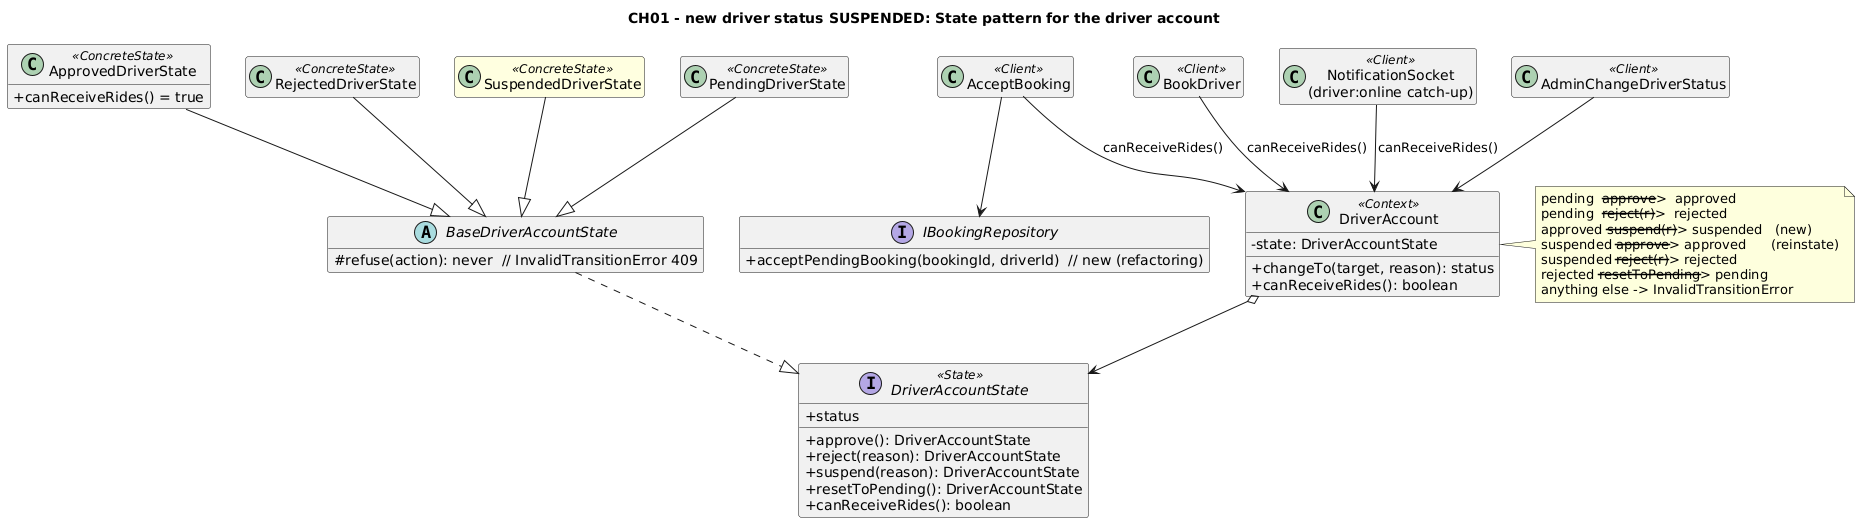
\includegraphics[width=0.8\linewidth]{Part2/diagrams/ch01_driver_account_state.png}\caption{CH01 State.}\end{figure}

\subsection*{CH02 -- Ride cancellation}
\textbf{Change and acceptance criteria:} riders and assigned drivers can cancel only their own PENDING or CONFIRMED rides; finished rides
return 409. Rider fee is 0 while PENDING or before 21:00 IST the day before, otherwise max(Rs~50, 10\% of the fare); driver
cancellations are free and notify the rider; unaccepted broadcasts dismiss the drivers' popups.\\
\textbf{Before and after:} \texttt{f635355} $\rightarrow$ \texttt{28a83c8}; 13 source files.\\
\textbf{Implementation and tests:} State (\texttt{TripLifecycle}) used by cancel, status update and expiry; Strategy
(\texttt{CancellationPolicy}) for the fee. \texttt{npm test}: 33/33 passed.\\
\textbf{Pattern effects:} two new instances; notification adapter, Observer, middleware chain, \texttt{catchAsync} decorator and trip
repository extended.\\
\textbf{Refactoring:} \emph{smells} -- a forced \texttt{status} parameter, cutoff arithmetic inside the use case, no status guard (the baseline test
\emph{a COMPLETED trip can still be cancelled} passed), no ownership check; \emph{techniques} -- Replace Conditional with State, Extract Class;
\emph{evidence} -- the baseline cancellation tests keep their expectations.\\
\textbf{Before/after metrics:} \texttt{CancelBooking} NLOC 48$\rightarrow$48 but max CC 5$\rightarrow$9 (ownership and recipient branches);
new \texttt{TripState.ts} 114 NLOC (max CC 4) and \texttt{CancellationPolicy.ts} 37 NLOC.

\begin{figure}[h]\centering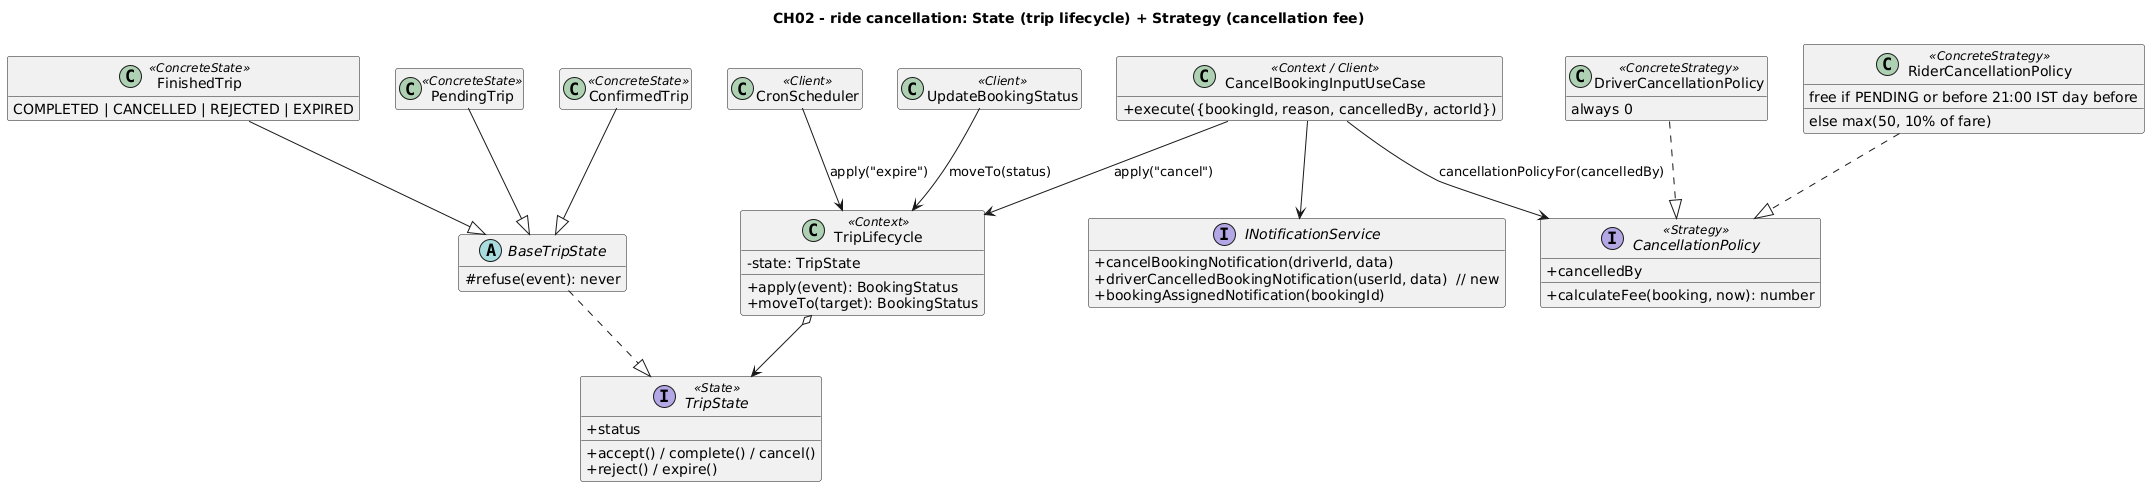
\includegraphics[width=0.8\linewidth]{Part2/diagrams/ch02_trip_state_cancellation.png}\caption{CH02 State + Strategy.}\end{figure}

\subsection*{CH03 -- Multiple ride types and dynamic pricing}
\textbf{Change and acceptance criteria:} new HOURLY (Rs~200 per started hour, min 4\,h) and OUTSTATION (Rs~12/km + Rs~300/day) ride types;
+25\% in peak hours (08:00--10:59, 17:00--20:59 IST) and +20\% when fewer than 3 drivers are in range; existing fares unchanged off-peak;
final fare uses each type's extra-km rate.\\
\textbf{Before and after:} \texttt{28a83c8} $\rightarrow$ \texttt{a12c878}; 7 source files.\\
\textbf{Implementation and tests:} Strategy per ride type in \texttt{domain/pricing/FareStrategy.ts}, Decorators in \texttt{DynamicPricing.ts},
\texttt{FareCalculatorService} as context; \texttt{BookDriver} prices after matching. \texttt{npm test}: 41/41 passed; the six baseline fare
tests pass unchanged.\\
\textbf{Pattern effects:} Ride Fare Pricing (Strategy) and Dynamic Fare Pricing (Decorator) newly introduced; DI extended.\\
\textbf{Refactoring:} \emph{smells} -- switch on \texttt{bookingType}, magic number \texttt{ratePerKm = 10} duplicated in \texttt{UpdateBookingStatus},
plain \texttt{Error} turning into HTTP 500; \emph{techniques} -- Replace Conditional with Polymorphism, Replace Magic Number;
\emph{evidence} -- unchanged characterization tests.\\
\textbf{Before/after metrics:} \texttt{FareCalculatorService} NLOC 32$\rightarrow$30, max CC 6$\rightarrow$2; \texttt{BookDriver} max CC 15$\rightarrow$18
(driver-state check and supply argument).

\begin{figure}[h]\centering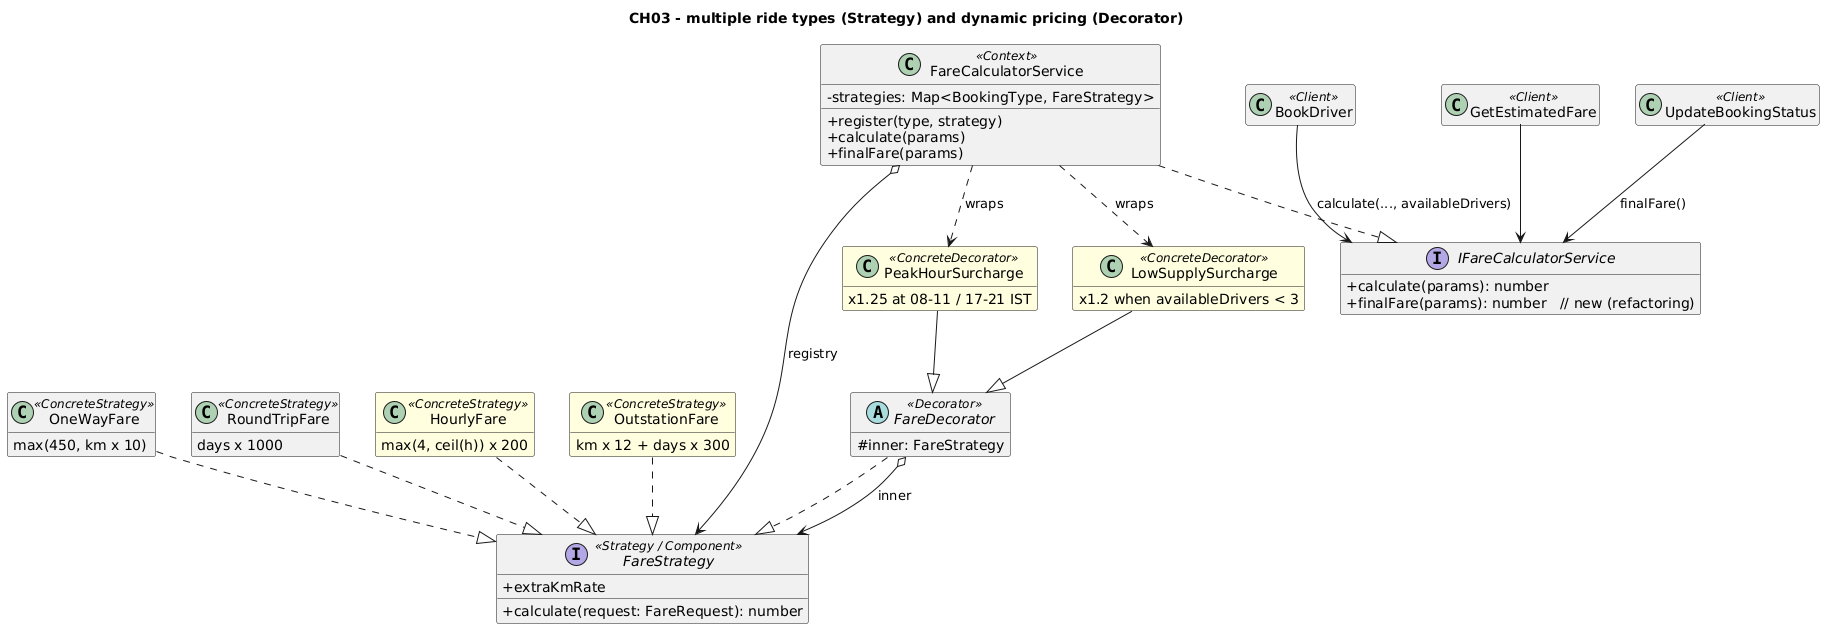
\includegraphics[width=0.9\linewidth]{Part2/diagrams/ch03_fare_strategy_decorator.png}\caption{CH03 Strategy + Decorator.}\end{figure}

\subsection*{Records of the newly introduced instances}

\subsubsection*{Driver Account Lifecycle}
\textbf{Pattern type and category:} State -- Behavioral.\\
\textbf{Purpose and origin:} Each status object answers which admin actions are legal and whether the driver may take rides. DriverAccount.changeTo maps the requested status to approve/reject/suspend/resetToPending on the current state, which returns the next state or throws InvalidTransitionError (409). Adding SUSPENDED needed one new class plus suspend() on ApprovedDriverState; tests: tests/driverStatus.test.ts (9 cases).

\noindent\begin{tabularx}{\linewidth}{@{}P{0.27\linewidth}Y@{}}
\toprule Pattern role & Actual class, interface or function \\ \midrule
State & DriverAccountState (+ BaseDriverAccountState default refusals) \\
ConcreteStates & PendingDriverState, ApprovedDriverState, RejectedDriverState, SuspendedDriverState \\
Context & DriverAccount \\
Clients & AdminChangeDriverStatus, AcceptBooking, BookDriver, NotificationSocket driver:online handler \\
\bottomrule
\end{tabularx}

\noindent\textbf{File and line ranges:}\begin{itemize}\setlength\itemsep{0pt}\item \texttt{Part2/\allowbreak{}code/\allowbreak{}src/\allowbreak{}domain/\allowbreak{}driver/\allowbreak{}DriverAccountState.\allowbreak{}ts:13-50}\item \texttt{Part2/\allowbreak{}code/\allowbreak{}src/\allowbreak{}domain/\allowbreak{}driver/\allowbreak{}DriverAccountState.\allowbreak{}ts:52-92}\item \texttt{Part2/\allowbreak{}code/\allowbreak{}src/\allowbreak{}domain/\allowbreak{}driver/\allowbreak{}DriverAccountState.\allowbreak{}ts:110-144}\item \texttt{Part2/\allowbreak{}code/\allowbreak{}src/\allowbreak{}application/\allowbreak{}use\_\allowbreak{}cases/\allowbreak{}Admin/\allowbreak{}AdminChangeDriverStatus.\allowbreak{}ts:31}\item \texttt{Part2/\allowbreak{}code/\allowbreak{}src/\allowbreak{}application/\allowbreak{}use\_\allowbreak{}cases/\allowbreak{}Driver/\allowbreak{}AcceptBooking.\allowbreak{}ts:29}\item \texttt{Part2/\allowbreak{}code/\allowbreak{}src/\allowbreak{}application/\allowbreak{}use\_\allowbreak{}cases/\allowbreak{}User/\allowbreak{}BookDriver.\allowbreak{}ts:48}\end{itemize}
\noindent\textbf{Verification:} Confirmed by unit tests listed in the change README.

\subsubsection*{Trip Lifecycle and Cancellation}
\textbf{Pattern type and category:} State -- Behavioral.\\
\textbf{Purpose and origin:} Trip transitions are decided by the current state object: PendingTrip accepts accept/cancel/reject/expire, ConfirmedTrip accepts complete/cancel/reject, FinishedTrip refuses everything. CancelBooking calls apply('cancel'), UpdateBookingStatus calls moveTo(status) and CronScheduler calls apply('expire'). Fixes the baseline defect where a COMPLETED trip could be cancelled; tests T1-T8 in tests/cancellation.test.ts.

\noindent\begin{tabularx}{\linewidth}{@{}P{0.27\linewidth}Y@{}}
\toprule Pattern role & Actual class, interface or function \\ \midrule
State & TripState (+ BaseTripState default refusals) \\
ConcreteStates & PendingTrip, ConfirmedTrip, FinishedTrip (COMPLETED/CANCELLED/REJECTED/EXPIRED) \\
Context & TripLifecycle \\
Clients & CancelBookingInputUseCase, UpdateBookingStatus, CronScheduler \\
\bottomrule
\end{tabularx}

\noindent\textbf{File and line ranges:}\begin{itemize}\setlength\itemsep{0pt}\item \texttt{Part2/\allowbreak{}code/\allowbreak{}src/\allowbreak{}domain/\allowbreak{}booking/\allowbreak{}TripState.\allowbreak{}ts:10-75}\item \texttt{Part2/\allowbreak{}code/\allowbreak{}src/\allowbreak{}domain/\allowbreak{}booking/\allowbreak{}TripState.\allowbreak{}ts:97-120}\item \texttt{Part2/\allowbreak{}code/\allowbreak{}src/\allowbreak{}application/\allowbreak{}use\_\allowbreak{}cases/\allowbreak{}User/\allowbreak{}CancelBooking.\allowbreak{}ts:35}\item \texttt{Part2/\allowbreak{}code/\allowbreak{}src/\allowbreak{}application/\allowbreak{}use\_\allowbreak{}cases/\allowbreak{}Driver/\allowbreak{}UpdateBookingstatus.\allowbreak{}ts:44}\item \texttt{Part2/\allowbreak{}code/\allowbreak{}src/\allowbreak{}infrastructure/\allowbreak{}services/\allowbreak{}CronScheduler.\allowbreak{}ts:30}\end{itemize}
\noindent\textbf{Verification:} Confirmed by unit tests listed in the change README.

\subsubsection*{Cancellation Fee Policy}
\textbf{Pattern type and category:} Strategy -- Behavioral.\\
\textbf{Purpose and origin:} The fee rule varies by who cancels. The rider policy is free while PENDING or before 21:00 IST the day before the ride, else max(Rs 50, 10\% of the estimated fare); the driver policy is always 0. The use case asks cancellationPolicyFor(cancelledBy) and calls calculateFee without knowing which rule runs.

\noindent\begin{tabularx}{\linewidth}{@{}P{0.27\linewidth}Y@{}}
\toprule Pattern role & Actual class, interface or function \\ \midrule
Strategy & CancellationPolicy \\
ConcreteStrategies & RiderCancellationPolicy, DriverCancellationPolicy \\
Selector & cancellationPolicyFor(cancelledBy) \\
Context & CancelBookingInputUseCase \\
\bottomrule
\end{tabularx}

\noindent\textbf{File and line ranges:}\begin{itemize}\setlength\itemsep{0pt}\item \texttt{Part2/\allowbreak{}code/\allowbreak{}src/\allowbreak{}domain/\allowbreak{}booking/\allowbreak{}CancellationPolicy.\allowbreak{}ts:6-9}\item \texttt{Part2/\allowbreak{}code/\allowbreak{}src/\allowbreak{}domain/\allowbreak{}booking/\allowbreak{}CancellationPolicy.\allowbreak{}ts:26-41}\item \texttt{Part2/\allowbreak{}code/\allowbreak{}src/\allowbreak{}domain/\allowbreak{}booking/\allowbreak{}CancellationPolicy.\allowbreak{}ts:43-50}\item \texttt{Part2/\allowbreak{}code/\allowbreak{}src/\allowbreak{}application/\allowbreak{}use\_\allowbreak{}cases/\allowbreak{}User/\allowbreak{}CancelBooking.\allowbreak{}ts:36}\end{itemize}
\noindent\textbf{Verification:} Confirmed by unit tests listed in the change README.

\subsubsection*{Ride Fare Pricing}
\textbf{Pattern type and category:} Strategy -- Behavioral.\\
\textbf{Purpose and origin:} One class per ride type computes the base fare and exposes its extra-km rate. FareCalculatorService looks the strategy up by bookingType; a new ride type is a new class plus one register() call. The 6 baseline characterization tests in tests/fare.test.ts still pass unchanged (behaviour preserved for ONE\_WAY/ROUND\_TRIP).

\noindent\begin{tabularx}{\linewidth}{@{}P{0.27\linewidth}Y@{}}
\toprule Pattern role & Actual class, interface or function \\ \midrule
Strategy & FareStrategy \\
ConcreteStrategies & OneWayFare, RoundTripFare, HourlyFare, OutstationFare \\
Context & FareCalculatorService (registry Map\textless{}BookingType, FareStrategy\textgreater{}, register()) \\
Clients & BookDriver, GetEstimatedFare, UpdateBookingStatus (finalFare) \\
\bottomrule
\end{tabularx}

\noindent\textbf{File and line ranges:}\begin{itemize}\setlength\itemsep{0pt}\item \texttt{Part2/\allowbreak{}code/\allowbreak{}src/\allowbreak{}domain/\allowbreak{}pricing/\allowbreak{}FareStrategy.\allowbreak{}ts:15-68}\item \texttt{Part2/\allowbreak{}code/\allowbreak{}src/\allowbreak{}infrastructure/\allowbreak{}services/\allowbreak{}FareCalculatorService.\allowbreak{}ts:10-35}\item \texttt{Part2/\allowbreak{}code/\allowbreak{}src/\allowbreak{}application/\allowbreak{}services/\allowbreak{}FareCalculatorService.\allowbreak{}ts:4-7}\item \texttt{Part2/\allowbreak{}code/\allowbreak{}src/\allowbreak{}application/\allowbreak{}use\_\allowbreak{}cases/\allowbreak{}User/\allowbreak{}BookDriver.\allowbreak{}ts:100-106}\item \texttt{Part2/\allowbreak{}code/\allowbreak{}src/\allowbreak{}application/\allowbreak{}use\_\allowbreak{}cases/\allowbreak{}Driver/\allowbreak{}UpdateBookingstatus.\allowbreak{}ts:60-64}\end{itemize}
\noindent\textbf{Verification:} Confirmed by unit tests listed in the change README.

\subsubsection*{Dynamic Fare Pricing}
\textbf{Pattern type and category:} Decorator -- Structural.\\
\textbf{Purpose and origin:} Pricing rules wrap any ride-type strategy with the same interface: PeakHourSurcharge multiplies by 1.25 for starts 08:00-10:59 and 17:00-20:59 IST, LowSupplySurcharge by 1.2 when fewer than 3 drivers are in range; they stack (60 km evening ride with 1 driver: 600 -\textgreater{} 750 -\textgreater{} 900). tests/pricing.test.ts.

\noindent\begin{tabularx}{\linewidth}{@{}P{0.27\linewidth}Y@{}}
\toprule Pattern role & Actual class, interface or function \\ \midrule
Component & FareStrategy \\
ConcreteComponents & OneWayFare/RoundTripFare/HourlyFare/OutstationFare \\
Decorator & FareDecorator (holds inner FareStrategy) \\
ConcreteDecorators & PeakHourSurcharge, LowSupplySurcharge \\
Client & FareCalculatorService.calculate (wraps the selected strategy) \\
\bottomrule
\end{tabularx}

\noindent\textbf{File and line ranges:}\begin{itemize}\setlength\itemsep{0pt}\item \texttt{Part2/\allowbreak{}code/\allowbreak{}src/\allowbreak{}domain/\allowbreak{}pricing/\allowbreak{}DynamicPricing.\allowbreak{}ts:7-40}\item \texttt{Part2/\allowbreak{}code/\allowbreak{}src/\allowbreak{}infrastructure/\allowbreak{}services/\allowbreak{}FareCalculatorService.\allowbreak{}ts:22-25}\item \texttt{Part2/\allowbreak{}code/\allowbreak{}src/\allowbreak{}domain/\allowbreak{}pricing/\allowbreak{}FareStrategy.\allowbreak{}ts:15-19}\end{itemize}
\noindent\textbf{Verification:} Confirmed by unit tests listed in the change README.


\subsection{Updated pattern counts}
\begin{tabular}{@{}lrrrl@{}}\toprule Snapshot & Types & Instances & Concrete classes & Rejected / uncertain (baseline scope)\\\midrule
Original code & 10 & 16 & 11 & 6 rejected, 2 uncertain \\
After CH01 & 11 & 17 & 15 & 6 rejected, 2 uncertain \\
After CH02 & 12 & 19 & 20 & 6 rejected, 2 uncertain \\
After CH03 & 12 & 21 & 26 & 6 rejected, 2 uncertain \\
\bottomrule\end{tabular}

No instance was removed or replaced; continuing collaborations keep their instance names. The Ride Fare Pricing Strategy replaces the
conditional that was the rejected Strategy candidate of the baseline, and the two State instances replace the status conditionals that
were the rejected State candidate.

\begin{longtable}{@{}P{0.09\linewidth}P{0.25\linewidth}P{0.16\linewidth}P{0.4\linewidth}@{}}
\caption{Instances whose status changed (all other rows: preserved; full table \texttt{data/patterns\_evolution.csv}).}\label{tab:evo}\\
\toprule Snapshot & Instance & Status & Change\\\midrule\endfirsthead
\toprule Snapshot & Instance & Status & Change\\\midrule\endhead
After CH01 & Ride Booking Request Flow (Layered Architecture) & modified & AcceptBooking no longer imports the Mongoose BookingModel (application -\textgreater{} infrastructure dependency removed); new domain module domain/driver holds the driver-account states. \\
After CH01 & Use-Case and Service Composition Root (Dependency Injection) & extended & AcceptBooking gains @inject(TOKENS.IDRIVER\_REPO); no new registrations needed. \\
After CH01 & Trip Booking Repository (Repository) & extended & New repository operation acceptPendingBooking (atomic PENDING-\textgreater{}CONFIRMED) moved out of AcceptBooking; AcceptBooking becomes a new client. \\
After CH01 & Driver Repository with Geospatial Matching Query (Repository) & modified & updateStatus accepts DriverAccountStatus (adds suspended) and stores the suspension reason; schema enum extended. The geo query is unchanged and already excludes non-approved (suspended) drivers. \\
After CH01 & Ride Event Notification (Observer) & modified & The driver:online subscription handler now skips the catch-up push for drivers whose account state cannot receive rides (pending/rejected/suspended); the admin status notification is sent only after a legal transition is saved. \\
After CH01 & Driver Account Lifecycle (State) & newly\_\allowbreak{}introduced & Requirement CH01 (new driver status). Replaces the any-to-any status update validated by an array includes() in AdminChangeDriverStatus (rejected State candidate in the baseline). \\
After CH02 & Trip Booking Repository (Repository) & extended & Booking entity and schema gain cancelledBy and cancellationFee, persisted through updateBooking by CancelBookingInputUseCase. \\
After CH02 & Socket.IO Ride Notification Adapter (Adapter) & extended & Target INotificationService gains driverCancelledBookingNotification; the adapter maps it to emit('booking:cancelledByDriver') on the rider socket. \\
After CH02 & Ride Event Notification (Observer) & extended & New published event booking:cancelledByDriver to riders; cancelling an unaccepted broadcast publishes booking:assigned so drivers dismiss the request. \\
After CH02 & Authenticated Ride Request Pipeline (Chain of Responsibility) & extended & New chain for drivers: protectRoute(['driver']) -\textgreater{} CheckBlockedUserOrDriver.handle -\textgreater{} BookingController.driverCancelBooking. \\
After CH02 & Async Controller Error Forwarding (Decorator) & extended & New ConcreteComponent driverCancelBooking wrapped by catchAsync; cancelBooking now reads the authenticated user id. \\
After CH02 & Trip Lifecycle and Cancellation (State) & newly\_\allowbreak{}introduced & Requirement CH02 (ride cancellation). Replaces scattered status if-checks in CancelBooking and UpdateBookingStatus. \\
After CH02 & Cancellation Fee Policy (Strategy) & newly\_\allowbreak{}introduced & Requirement CH02. The baseline cutoff rule (refuse after 21:00 IST) moved from CancelBooking into RiderCancellationPolicy and became a late fee. \\
After CH03 & Use-Case and Service Composition Root (Dependency Injection) & extended & UpdateBookingStatus gains @inject(TOKENS.IFARE\_CALCULATE\_SERVICE). \\
After CH03 & Ride Fare Pricing (Strategy) & newly\_\allowbreak{}introduced & Requirement CH03 (multiple ride types). Replaces the if/else in FareCalculatorService.calculate (the rejected Strategy candidate of the baseline) and the duplicated ratePerKm = 10 in UpdateBookingStatus. \\
After CH03 & Dynamic Fare Pricing (Decorator) & newly\_\allowbreak{}introduced & Requirement CH03 (dynamic pricing). BookDriver now prices after matching so availableDrivers is known. \\
\bottomrule
\end{longtable}

\textbf{Same-scope metrics of the edited and new files after CH03} (\texttt{tools/ts\_metrics.js}; NLOC = non-blank, non-comment lines):
\begin{longtable}{@{}P{0.7\linewidth}rr@{}}\toprule File & NLOC & max CC\\\midrule\endhead
\texttt{application/\allowbreak{}use\_\allowbreak{}cases/\allowbreak{}Admin/\allowbreak{}AdminChangeDriverStatus.\allowbreak{}ts} & 32 & 3 \\
\texttt{application/\allowbreak{}use\_\allowbreak{}cases/\allowbreak{}Driver/\allowbreak{}AcceptBooking.\allowbreak{}ts} & 58 & 6 \\
\texttt{application/\allowbreak{}use\_\allowbreak{}cases/\allowbreak{}User/\allowbreak{}CancelBooking.\allowbreak{}ts} & 48 & 9 \\
\texttt{application/\allowbreak{}use\_\allowbreak{}cases/\allowbreak{}Driver/\allowbreak{}UpdateBookingstatus.\allowbreak{}ts} & 64 & 12 \\
\texttt{infrastructure/\allowbreak{}services/\allowbreak{}FareCalculatorService.\allowbreak{}ts} & 30 & 2 \\
\texttt{application/\allowbreak{}use\_\allowbreak{}cases/\allowbreak{}User/\allowbreak{}BookDriver.\allowbreak{}ts} & 136 & 18 \\
\texttt{infrastructure/\allowbreak{}services/\allowbreak{}CronScheduler.\allowbreak{}ts} & 45 & 5 \\
\texttt{domain/\allowbreak{}driver/\allowbreak{}DriverAccountState.\allowbreak{}ts} & 135 & 6 \\
\texttt{domain/\allowbreak{}booking/\allowbreak{}TripState.\allowbreak{}ts} & 114 & 4 \\
\texttt{domain/\allowbreak{}booking/\allowbreak{}CancellationPolicy.\allowbreak{}ts} & 37 & 4 \\
\texttt{domain/\allowbreak{}pricing/\allowbreak{}FareStrategy.\allowbreak{}ts} & 52 & 3 \\
\texttt{domain/\allowbreak{}pricing/\allowbreak{}DynamicPricing.\allowbreak{}ts} & 28 & 5 \\
\bottomrule\end{longtable}
Whole \texttt{src}: 8{,}232 NLOC / 399 functions before, 8{,}680 NLOC / 460 functions after; maximum function CC 17 $\rightarrow$ 18.

\textbf{Interpretation:} the new states and strategies made each requirement an additive change: SUSPENDED is one new class and one
method, a new ride type or pricing rule is one class plus a registration, and illegal transitions are refused in one place. The cost is
about 450 more NLOC and more, smaller functions; some use cases (\texttt{CancelBooking}, \texttt{BookDriver}) gained complexity because they
now enforce ownership and supply rules. More or fewer LOC alone does not prove a better design; the evidence for the improvement is
that two baseline defects are now caught by tests and that the old fare behaviour is preserved by unchanged tests. Remaining limitations:
\texttt{UpdateBookingStatus} still does not check that the caller is the booking's driver; the pre-booking estimate cannot include the
low-supply surcharge; cancellation is still read-then-update rather than one atomic conditional update, and acceptance does not re-check
\texttt{activePayment} -- the last two were pointed out by the ChatGPT reviews in Section~\ref{sec:llm} and are left as future work.

%=====================================================================
\section{Part 3 Cross-language comparison}
\textbf{Selected instances:} Ride Fare Pricing (Strategy, CH03), Trip Lifecycle and Cancellation (State, CH02), Ride Event Notification
(Observer, baseline). These are the patterns the requirements changed most; the infrastructure patterns (Repository, Adapter, Gateway,
Data Mapper, DI) depend on MongoDB, Stripe, Google or tsyringe and have no self-contained four-language equivalent with identical behaviour.

\textbf{Common specifications:} \texttt{Part3/test-cases/strategy\_spec.md} (S1--S8: fares for every ride type, invalid input, unknown type),
\texttt{state\_spec.md} (T1--T8: event sequences, final state and number of refused events), \texttt{observer\_spec.md} (O1--O6:
broadcast, unsubscribe, reconnect replacement, ordering). S1--S8 and T1--T8 are also asserted against the TypeScript code.

\textbf{Implementations:} \texttt{Part3/<pattern>/\{java,python,javascript,cpp\}/} -- Java 25, Python 3.13.7, Node.js 22.18.0, g++ 13.5.0
(\texttt{-std=c++20 -O2}, Docker \texttt{gcc:13}); commands in each folder's README and \texttt{tools/run\_part3.py}.

\textbf{Actual results and static/dynamic comparison} (\texttt{data/cross\_language.csv}; LOC = lizard NLOC of the production file;
CC = maximum function cyclomatic complexity; time = median of 5 complete test processes after 1 warm-up):

\begin{tabular}{@{}llrrlr@{}}\toprule Pattern & Language & LOC & max CC & Tests & Median ms\\\midrule
Strategy & Java & 57 & 3 & 8/8 passed & 102.7 \\
Strategy & Python & 51 & 3 & 8/8 passed & 59.8 \\
Strategy & JavaScript & 47 & 3 & 8/8 passed & 49.4 \\
Strategy & C++ & 69 & 3 & 8/8 passed & 2.1 \\
State & Java & 58 & 6 & 8/8 passed & 98.3 \\
State & Python & 52 & 2 & 8/8 passed & 31.0 \\
State & JavaScript & 41 & 2 & 8/8 passed & 45.3 \\
State & C++ & 57 & 6 & 8/8 passed & 1.9 \\
Observer & Java & 33 & 3 & 6/6 passed & 110.8 \\
Observer & Python & 31 & 3 & 6/6 passed & 63.5 \\
Observer & JavaScript & 24 & 2 & 6/6 passed & 46.3 \\
Observer & C++ & 40 & 3 & 6/6 passed & 2.3 \\
\bottomrule\end{tabular}

All 12 implementations passed every fixture. Times include process start-up and are dominated by it (JVM about 100\,ms, Node about 47\,ms,
CPython 31--64\,ms, native C++ about 2\,ms measured inside the container); they are not throughput benchmarks.

\textbf{Comparison:}
\begin{longtable}{@{}P{0.2\linewidth}P{0.76\linewidth}@{}}\toprule Snippet & Observed language-specific structure\\\midrule\endhead
Strategy / Java & Nominal FareStrategy interface plus nested static classes and a Trip record; the compiler rejects a strategy that lacks calculate(). HashMap registry in the context. Median dominated by JVM start-up (\textasciitilde{}100 ms). \\
Strategy / Python & typing.Protocol gives a structural interface that is only checked by a type checker, not at runtime; frozen dataclass for the trip. Importing dataclasses/typing roughly doubles start-up versus the State snippet (60 vs 31 ms). \\
Strategy / JavaScript & Duck typing: any object with calculate(trip) is accepted; a private \#strategies Map holds the registry. ES module; the role names exist only as class names. \\
Strategy / C++ & Abstract base class with pure virtual calculate(); the context owns strategies through std::unique\_ptr in a std::map, so ownership is explicit. Header-only snippet compiled with -O2; native binary starts in \textasciitilde{}2 ms (measured inside the container). \\
State / Java & Interface + abstract BaseState supplying refusing defaults, concrete states as nested classes; the context maps event names with a switch expression, which gives the highest function CC (6). \\
State / Python & Base class with refusing methods; concrete states override; the context dispatches with getattr(state, event)(), so no branch per event (CC 2). No typing/dataclass imports, hence the fastest Python start-up (31 ms). \\
State / JavaScript & Same shape as Python: class inheritance for default refusals and dynamic dispatch with state[event](); class fields hold the state name. \\
State / C++ & Virtual methods returning std::unique\_ptr\textless{}TripState\textgreater{}; [[noreturn]] refuse() in the base. The context owns the current state and replaces it on each transition; event dispatch is an if-chain (CC 6) because C++ has no reflective method lookup. \\
Observer / Java & Observer interface, RecordingObserver collecting events in a List and a HashMap subscriber registry; lambdas in the test runner. Static typing forces every observer to implement update(). \\
Observer / Python & Protocol for Observer and a dict registry; broadcast is a one-line generator sum. Observers need no common base class at runtime. \\
Observer / JavaScript & Any object with update() can subscribe; Map registry and Array.filter for broadcast give the smallest source (24 LOC) and lowest CC (2). \\
Observer / C++ & Hub stores std::weak\_ptr so it never extends an observer's lifetime; notify() locks the pointer and skips destroyed observers - an ownership question the garbage-collected languages do not need to answer. \\
\bottomrule\end{longtable}

\textbf{Technology discussion:} Java and C++ express the pattern roles as nominal types checked by the compiler (interfaces, abstract
classes, \texttt{override}); Python \texttt{Protocol}s and JavaScript duck typing make the same roles conventions, so the code is shorter
but a missing method is found only when it runs. Dynamic dispatch by name (\texttt{getattr}, \texttt{state[event]()}) removed the event
switch in Python/JS (CC 2 versus 6 in Java/C++), which matches the GoF observation that State replaces conditionals with polymorphism but
the context still needs a way to map events to methods. C++ is the only version that must state ownership: the Strategy context owns
strategies through \texttt{unique\_ptr}, the State context replaces its state object, and the Observer hub keeps \texttt{weak\_ptr}s so a
subscription never keeps a disconnected observer alive -- a concern garbage-collected runtimes hide. (Sources: Gamma et al.\ 1994; Python
\texttt{typing.Protocol} PEP 544; ISO C++ smart-pointer guidelines.)

%=====================================================================
\section{LLM records and human verification}\label{sec:llm}
\textbf{Run and model:} 10 real runs on 2026-10-11. (a) Dilip Kumar Reddy's prompt to Claude Opus 5.5 in the Claude Code desktop app (paid tier,
not a free tool) for the application study and first pattern list (\texttt{prompts/Dilip\_Kumar\_Reddy\_claude\_*}). (b) Nine prompts on
\textbf{ChatGPT, free tier, logged out} (the interface shows no model name). Members were unavailable, so with the team lead's approval each
prompt file was pasted unchanged into a new chat from his computer, with the browser driven by Claude Code; the member named on a file is the
owner of that topic, not the person who typed it. Prompts embed the exact source excerpts, specifications or CSVs the model received.

\textbf{Inputs and outputs:} prompt, input, raw output and verification paths are in \texttt{data/llm.csv}; inputs come from the baseline
commit c8766f4 (\texttt{Part1/code}) or from our own specifications and datasets. Outputs were captured from the rendered page and converted
to Markdown without editing the content.

\textbf{Claims and evaluation:}
\begin{longtable}{@{}P{0.17\linewidth}P{0.14\linewidth}P{0.12\linewidth}P{0.5\linewidth}@{}}\toprule Part & Topic owner & Model & Evaluation (details in the verification file)\\\midrule\endhead
Pattern discovery (application study) & Dilip Kumar Reddy & Claude Opus 5.5 & Partially correct: Repository, DI, Singleton, Adapter (Socket.IO, Stripe), Observer, Chain of Responsibility, Data Mapper and Layered Architecture were confirmed; Twilio/Cloudinary adapters are unused or out of scope; Gateway and catchAsync Decorator were missed; ON\_TRIP proposal was replaced by SUSPENDED. \\
Pattern discovery & Dilip Kumar Reddy & ChatGPT free & Partial: agrees on Repository, DI, Layered Architecture, Adapter, middleware chain and on all 6 rejected candidates; disputes our Observer, catchAsync Decorator and module Singleton; Data Mapper and Gateway code was not in the excerpt. \\
Evolution CH01 (new driver status) & Sai Sameer & ChatGPT free & Correct defect analysis (5/5 baseline defects confirmed); partial design: its 'State' is a transition table, not state objects; it flags an activePayment check and a suspend/accept race that remain open in our CH01. \\
Cross-language analysis (Observer) & Sai Sameer & ChatGPT free & Partial: all 4 generated implementations compile and pass O1-O6; verbosity ranking wrong for its own Java/C++; its C++ hub keeps observers alive with shared\_ptr (ours uses weak\_ptr). \\
Evolution CH02 (ride cancellation) & M Kumar & ChatGPT free & Partial: accurate defects including the non-atomic read-then-update, which is still present in our CH02; recommends Strategy (matches ours) but advises against State (we chose State); one formula glitch and one unsafe driverId! sample. \\
Cross-language analysis (State) & M Kumar & ChatGPT free & Correct: all 4 generated implementations pass T1-T8; size ranking matches its code; 'same complexity' claim only partly true (max CC 2-4 vs 6). \\
Evolution CH03 (ride types and dynamic pricing) & K Harish & ChatGPT free & Partial: smells and Strategy design match our CH03; rule pipeline instead of our Decorator (equivalent x1.5 stacking); km-validation 'defect' already handled by Zod schema; hourly billing not rounded to started hours. \\
Cross-language analysis (Strategy) & K Harish & ChatGPT free & Partial: all 4 generated implementations pass S1-S8; comparison table wrongly lists inheritance for its JS; size ranking holds only when tests are inside the files. \\
Pattern discovery (dataset audit) & S Leela Shankar & ChatGPT free & Correct: counts and participant roles confirmed with no errors; its caveats (Observer combined roles, framework CoR, function Decorator) are already recorded in the dataset. \\
Cross-language analysis (metrics) & S Leela Shankar & ChatGPT free & Correct: reproduces every number and gives sound threats to validity; two minor slips (CC remark; says raw timings are missing although they are in Part3/evidence). \\
\bottomrule\end{longtable}

\textbf{What the evaluation showed:} 3 runs correct, 7 partially correct, none fully incorrect. All 12 programs that ChatGPT generated for the
cross-language prompts compiled and passed every fixture (\texttt{prompts/*\_coderun\_02.txt}), but its explanations made factual slips about its
own code (a JavaScript ``inheritance'' entry, size rankings). In pattern discovery it agreed with our Repository, DI, Layered, Adapter and
middleware-chain findings and with all six rejected candidates, but disputed three of our classifications (Observer with remote observers,
the function-wrapper Decorator \texttt{catchAsync}, the module-level Singleton); we keep them with their caveats stated in the records. For the
change requests it proposed the same Strategy designs, preferred a transition table or a single eligibility check where we used State, and
found two weaknesses that remain in our implementation (non-atomic cancellation, no \texttt{activePayment} check on acceptance). A model
statement was never accepted without code or test evidence.

\textbf{Generated code in our deliverables:} the TypeScript changes and the Part 3 snippets were written with AI assistance in the Claude Code session
and are accepted only through the evidence in this report: 41 application tests, 22 fixtures per language set, \texttt{tsc} with no new errors and
\texttt{-Wall -Wextra -Wpedantic} with no warnings. Each topic owner reviews their part and signs \texttt{HUMAN\_VERIFICATION.md}.

%=====================================================================
\section{Findings, contributions and references}
\textbf{Findings:} (1) The baseline already uses a clean, interface-first architecture: 16 collaborations of 10 pattern types, dominated by
Repository (5) and Adapter (3) instances made possible by tsyringe DI. (2) Its variability points were conditionals: ride-type pricing and
both status lifecycles had no behavioural pattern, and two defects followed from that (a completed trip could be cancelled; an admin could
jump a rejected driver to approved). (3) The four requirements introduced two State, two Strategy and one Decorator instance and extended
the notification Adapter/Observer, ending at 12 types and 21 instances with no removals. (4) Across languages the pattern structure stays the
same; what changes is how roles are declared (nominal vs structural), how events are dispatched, and whether ownership must be explicit.
(5) The LLM was useful as a reviewer -- it confirmed most findings and exposed two remaining weaknesses -- but 7 of 10 answers needed correction,
so its statements served as hypotheses to verify, not as evidence.
Limitations: no live end-to-end run against external services; dependency drift; no upstream license; client-side observers out of scope.

\textbf{Contributions} (\texttt{data/contributions.csv}):\\
\begin{tabular}{@{}P{0.2\linewidth}P{0.74\linewidth}@{}}\toprule Member & Contribution and evidence\\\midrule
Dilip Kumar Reddy & Lead: application study, architecture, Part 1 discovery, integration, report, submission; \texttt{Part1/}, \texttt{data/patterns.csv}, \texttt{README.md}\\
Sai Sameer & CH01 new driver status (State) and Part 3 Observer; \texttt{Part2/changes/CH01}, \texttt{Part3/observer\_ride\_notification}\\
M Kumar & CH02 ride cancellation (State, Strategy) and Part 3 State; \texttt{Part2/changes/CH02}, \texttt{Part3/state\_trip\_lifecycle}\\
K Harish & CH03 ride types and dynamic pricing (Strategy, Decorator) and Part 3 Strategy; \texttt{Part2/changes/CH03}, \texttt{Part3/strategy\_ride\_fare}\\
S Leela Shankar & UML diagrams, Part 3 measurement harness and cross-language metrics, dataset audit, slides; \texttt{Part1/diagrams}, \texttt{Part2/diagrams}, \texttt{Part3/evidence}, \texttt{tools/run\_part3.py}\\
\bottomrule\end{tabular}

\textbf{References:}
\begin{enumerate}
\item AkhilMM2000, \emph{sarathi-backend}, \url{https://github.com/AkhilMM2000/sarathi-backend}, commit c8766f4.
\item E.~Gamma, R.~Helm, R.~Johnson, J.~Vlissides, \emph{Design Patterns: Elements of Reusable Object-Oriented Software}, Addison-Wesley, 1994.
\item M.~Fowler, \emph{Patterns of Enterprise Application Architecture}, Addison-Wesley, 2002 (Repository, Data Mapper, Gateway).
\item M.~Fowler, \emph{Refactoring}, 2nd ed., Addison-Wesley, 2018.
\item Express 4 middleware guide, \url{https://expressjs.com/en/guide/using-middleware.html}; tsyringe, \url{https://github.com/microsoft/tsyringe};
Socket.IO v4 documentation, \url{https://socket.io/docs/v4/}.
\item PEP 544 -- Protocols: structural subtyping, \url{https://peps.python.org/pep-0544/}.
\item Tools: lizard 1.17.13, PlantUML 1.2024.7, Node test runner, Docker \texttt{gcc:13}.
\end{enumerate}

%=====================================================================
\section{Team folder and datasets}
\begin{verbatim}
A6/
  README.md  HUMAN_VERIFICATION.md  A6_Report.tex  A6_Report.pdf
  data/    patterns.csv, pattern_counts.csv, patterns_evolution.csv,
           cross_language.csv, llm.csv, contributions.csv
  Part1/   code/, diagrams/, evidence/, llm/
  Part2/   code/, changes/CH01..CH03/, diagrams/, evidence/, llm/
  Part3/   strategy_ride_fare/, state_trip_lifecycle/, observer_ride_notification/,
           test-cases/, evidence/, llm/, A6_slide.pdf
  prompts/ tools/
\end{verbatim}
Screenshot of the team folder in the GitHub fork: to be added after upload.

\end{document}
